% This file was converted to LaTeX by Writer2LaTeX ver. 1.0.2
% see http://writer2latex.sourceforge.net for more info
\documentclass[letterpaper]{article}
\usepackage[ascii]{inputenc}
\usepackage[T1]{fontenc}
\usepackage[portuges,english,english]{babel}
\usepackage{amsmath}
\usepackage{amssymb,amsfonts,textcomp}
\usepackage{color}
\usepackage{array}
\usepackage{hhline}
\usepackage{hyperref}
\hypersetup{pdftex, colorlinks=true, linkcolor=blue, citecolor=blue, filecolor=blue, urlcolor=blue, pdftitle=, pdfauthor=Bruno Azevedo, pdfsubject=, pdfkeywords=}
\usepackage[pdftex]{graphicx}
% Text styles
\newcommand\textstyleStrongEmphasis[1]{\textbf{#1}}
% Outline numbering
\setcounter{secnumdepth}{0}
% List styles
\newcommand\liststyleLi{%
\renewcommand\labelitemi{{\textbullet}}
\renewcommand\labelitemii{[27A2?]}
\renewcommand\labelitemiii{{\textbullet}}
\renewcommand\labelitemiv{{\textbullet}}
}
\newcommand\liststyleLii{%
\renewcommand\labelitemi{[27A2?]}
\renewcommand\labelitemii{[27A2?]}
\renewcommand\labelitemiii{[27A2?]}
\renewcommand\labelitemiv{[27A2?]}
}
\newcommand\liststyleLiii{%
\renewcommand\labelitemi{[27A2?]}
\renewcommand\labelitemii{[27A2?]}
\renewcommand\labelitemiii{[27A2?]}
\renewcommand\labelitemiv{[27A2?]}
}
\newcommand\liststyleLiv{%
\renewcommand\labelitemi{[27A2?]}
\renewcommand\labelitemii{[27A2?]}
\renewcommand\labelitemiii{[27A2?]}
\renewcommand\labelitemiv{[27A2?]}
}
\newcommand\liststyleLv{%
\renewcommand\labelitemi{[27A2?]}
\renewcommand\labelitemii{[27A2?]}
\renewcommand\labelitemiii{[27A2?]}
\renewcommand\labelitemiv{[27A2?]}
}
\newcommand\liststyleLvi{%
\renewcommand\labelitemi{[27A2?]}
\renewcommand\labelitemii{[27A2?]}
\renewcommand\labelitemiii{[27A2?]}
\renewcommand\labelitemiv{[27A2?]}
}
\newcommand\liststyleLvii{%
\renewcommand\labelitemi{[27A2?]}
\renewcommand\labelitemii{[27A2?]}
\renewcommand\labelitemiii{[27A2?]}
\renewcommand\labelitemiv{[27A2?]}
}
\newcommand\liststyleLviii{%
\renewcommand\labelitemi{[27A2?]}
\renewcommand\labelitemii{[27A2?]}
\renewcommand\labelitemiii{[27A2?]}
\renewcommand\labelitemiv{[27A2?]}
}
\newcommand\liststyleLix{%
\renewcommand\labelitemi{[27A2?]}
\renewcommand\labelitemii{[27A2?]}
\renewcommand\labelitemiii{[27A2?]}
\renewcommand\labelitemiv{[27A2?]}
}
\newcommand\liststyleLx{%
\renewcommand\labelitemi{[27A2?]}
\renewcommand\labelitemii{[27A2?]}
\renewcommand\labelitemiii{[27A2?]}
\renewcommand\labelitemiv{[27A2?]}
}
\newcommand\liststyleLxi{%
\renewcommand\labelitemi{[27A2?]}
\renewcommand\labelitemii{[27A2?]}
\renewcommand\labelitemiii{[27A2?]}
\renewcommand\labelitemiv{[27A2?]}
}
\newcommand\liststyleLxii{%
\renewcommand\labelitemi{[27A2?]}
\renewcommand\labelitemii{[27A2?]}
\renewcommand\labelitemiii{[27A2?]}
\renewcommand\labelitemiv{[27A2?]}
}
\newcommand\liststyleLxiii{%
\renewcommand\labelitemi{[27A2?]}
\renewcommand\labelitemii{[27A2?]}
\renewcommand\labelitemiii{[27A2?]}
\renewcommand\labelitemiv{[27A2?]}
}
\newcommand\liststyleLxiv{%
\renewcommand\labelitemi{[27A2?]}
\renewcommand\labelitemii{[27A2?]}
\renewcommand\labelitemiii{[27A2?]}
\renewcommand\labelitemiv{[27A2?]}
}
\newcommand\liststyleLxv{%
\renewcommand\labelitemi{{\textbullet}}
\renewcommand\labelitemii{{\textbullet}}
\renewcommand\labelitemiii{{\textbullet}}
\renewcommand\labelitemiv{{\textbullet}}
}
\newcommand\liststyleLxvi{%
\renewcommand\labelitemi{{\textbullet}}
\renewcommand\labelitemii{{\textbullet}}
\renewcommand\labelitemiii{{\textbullet}}
\renewcommand\labelitemiv{{\textbullet}}
}
\newcommand\liststyleLxvii{%
\renewcommand\labelitemi{[27A2?]}
\renewcommand\labelitemii{[27A2?]}
\renewcommand\labelitemiii{[27A2?]}
\renewcommand\labelitemiv{[27A2?]}
}
\newcommand\liststyleLxviii{%
\renewcommand\labelitemi{{\textbullet}}
\renewcommand\labelitemii{{\textbullet}}
\renewcommand\labelitemiii{{\textbullet}}
\renewcommand\labelitemiv{{\textbullet}}
}
\newcommand\liststyleLxix{%
\renewcommand\labelitemi{[27A2?]}
\renewcommand\labelitemii{[27A2?]}
\renewcommand\labelitemiii{[27A2?]}
\renewcommand\labelitemiv{[27A2?]}
}
\newcommand\liststyleLxx{%
\renewcommand\labelitemi{[27A2?]}
\renewcommand\labelitemii{[27A2?]}
\renewcommand\labelitemiii{[27A2?]}
\renewcommand\labelitemiv{[27A2?]}
}
% Page layout (geometry)
\setlength\voffset{-1in}
\setlength\hoffset{-1in}
\setlength\topmargin{0.7874in}
\setlength\oddsidemargin{0.7874in}
\setlength\textheight{9.4251995in}
\setlength\textwidth{6.9251995in}
\setlength\footskip{0.0cm}
\setlength\headheight{0cm}
\setlength\headsep{0cm}
% Footnote rule
\setlength{\skip\footins}{0.0469in}
\renewcommand\footnoterule{\vspace*{-0.0071in}\setlength\leftskip{0pt}\setlength\rightskip{0pt plus 1fil}\noindent\textcolor{black}{\rule{0.25\columnwidth}{0.0071in}}\vspace*{0.0398in}}
% Pages styles
\makeatletter
\newcommand\ps@Standard{
  \renewcommand\@oddhead{}
  \renewcommand\@evenhead{}
  \renewcommand\@oddfoot{}
  \renewcommand\@evenfoot{}
  \renewcommand\thepage{\arabic{page}}
}
\makeatother
\pagestyle{Standard}
% footnotes configuration
\makeatletter
\renewcommand\thefootnote{\arabic{footnote}}
\makeatother
\title{}
\author{Bruno Azevedo}
\date{2012-07-24}
\begin{document}
\subsection[Base de Dados]{\selectlanguage{english} Base de Dados}
{\selectlanguage{english}
Neste cap\'itulo, iremos apresentar uma contextualiza\c{c}\~ao sobre a
necessidade desta base de dados e a nossa solu\c{c}\~ao final de base
de dados. Para isso, enunciaremos as tabelas criadas e explicaremos a
sua raz\~ao de ser.}


\bigskip

\subsubsection[Contextualiza\c{c}\~ao]{\selectlanguage{english}
Contextualiza\c{c}\~ao}
{\selectlanguage{english}
Uma das funcionalidades exigidas neste projeto \'e o arquivamento do
esp\'olio do museu. \ Arquivar o esp\'olio significa receber
meta-informa\c{c}\~ao sobre cada objeto do esp\'olio (eventualmente o
pr\'oprio objeto se ele for digital), classific\'a-lo \`a luz de uma
ontologia definida \`a partida (mas que poder\'a ir evoluindo) e
armazenar a meta-informa\c{c}\~ao ap\'os classifica\c{c}\~ao. }

{\selectlanguage{english}
Outra grande funcionalidade exigida \'e a \ gera\c{c}\~ao autom\'atica
de espa\c{c}os de aprendizagem na forma de salas de exposi\c{c}\~ao do
museu. \ Cada sala de exposi\c{c}\~ao de um Museu Virtual (MV) \'e um
s\'itio Web atrav\'es do qual se podem ver os objetos em
exposi\c{c}\~ao, ou a sua descri\c{c}\~ao, devidamente relacionados
entre si de forma a transmitir o conhecimento correspondente ao tema
dessa exposi\c{c}\~ao. Estes espa\c{c}os de aprendizagem tamb\'em
necessitam de ser armazenados.}

{\selectlanguage{english}
Finalmente, a terceira grande funcionalidade passa por guiar as visitas
pelas salas de exposi\c{c}\~ao recebendo delas informa\c{c}\~ao.
\ Guiar a visita significa apresentar o s\'itio criado com base na
ontologia da exposi\c{c}\~ao e as indica\c{c}\~oes relativas \`a
disposi\c{c}\~ao dos objetos na sala e permitir que o visitante da
p\'agina possa deixar coment\'arios.}


\bigskip

{\selectlanguage{english}
O reposit\'orio que ir\'a armazenar toda esta informa\c{c}\~ao, ser\'a
constitu\'ido por uma base de dados relacional assim como num conjunto
de diretorias no servidor da aplica\c{c}\~ao. Neste cap\'itulo,
ir-nos-emos focar no desenvolvimento da base de dados.}

{\selectlanguage{english}
A especifica\c{c}\~ao do modelo de dados relacional foi baseado no
estudo das seguintes normas \textit{Categories for the Description of
Works of Art (CDWA)} e \textit{Cataloging Cultural Objects (CCO) }e
\textit{CDWA Lite}. \ }

{\selectlanguage{english}
O CDWA descreve o conte\'udo de bases de dados de arte articulando uma
\textit{framework} conceptual para descrever e aceder a
informa\c{c}\~ao sobre obras de arte, arquitetura, outro materiais de
cultura, grupos e cole\c{c}\~oes de obras e imagens relacionadas. O
CDWA inclui 532 categorias e subcategorias. }

{\selectlanguage{english}
O CCO \'e um guia ao inv\'es de um conjunto de elementos de meta-dados.
Os elementos que abrange s\~ao referentes a \'areas de informa\c{c}\~ao
num registo de cataloga\c{c}\~ao que podem ser mapeadas para v\'arios
elementos de meta-dados tais como CDWA ou CDWA Lite. Basicamente, \'e
um documento lato que inclui regras para formata\c{c}\~ao de dados,
sugest\~oes para informa\c{c}\~ao obrigat\'oria, requisitos para
vocabul\'ario controlado e problemas de apresenta\c{c}\~ao.}

{\selectlanguage{english}
Para facilitar a partilha de registos complacentes com CDWA atrav\'es do
protocolo \textit{Open Archives Initiative -- Protocol for Metadata
Harvesting (OAI-PMH)}, o Getty Research Institute criou o schema \ XML
CDWA Lite baseado nas categorias consideradas essenciais (core) do CDWA
que descreve um formato para registos essenciais de obras de arte e
material cultural baseados no CDWA e CCO.}


\bigskip

{\selectlanguage{english}
Ap\'os uma an\'alise a todas estas normas e estruturas, cheg\'amos a um
modelo final que passaremos a descrever na sec\c{c}\~ao seguinte.}


\bigskip


\bigskip

\subsubsection[Modelo de Dados]{\selectlanguage{english} Modelo de
Dados}
{\selectlanguage{english}
O modelo representa uma simplifica\c{c}\~ao do que \'e sugerido pelo
CDWA, apenas representando os meta-dados core e outros que ach\'amos
que seriam interessantes e importantes para a descri\c{c}\~ao de uma
obra de arte. Trata-se ent\~ao de uma estrutura capaz de representar
tudo que \'e necess\'ario para cobrir os requisitos apresentados.}


\bigskip

{\selectlanguage{english}
Para representar a primeira funcionalidade enunciada anteriormente,
descreveremos cada uma das tabelas criadas assim como a(s) categoria(s)
do CDWA que pretendem representar.}


\bigskip

{\selectlanguage{english}
As chaves prim\'arias s\~ao representadas por atributos sublinhados e as
chaves estrangeiras por atributos em it\'alico.}


\bigskip

\paragraph[Tabelas com origem em entidades e relacionamentos
1:N]{\selectlanguage{english} Tabelas com origem em entidades e
relacionamentos 1:N}
{\selectlanguage{english}
As seguintes tabelas foram criadas com base nos meta-dados que
pretendemos armazenar:}

\liststyleLi
\begin{itemize}
\item {\selectlanguage{english}
\textbf{Object\_Work\_Records} \{id\_object\_Work\_Records,
displayCreator, displayMeasurements, displayMaterialsTech,
displayCreationDate, \textit{RecordType}\}}

\foreignlanguage{english}{Correspondente \`a categoria
}\textstyleStrongEmphasis{\foreignlanguage{english}{Object/Work}}\textstyleStrongEmphasis{\foreignlanguage{english}{\textmd{.
Esta tabela identifica o foco l\'ogico da discuss\~ao. Representa uma
obra de arte (objeto) no reposit\'orio, descreve o que \'e a obra e
possibilita a procura de obras de um determinados tipo.}}}


\bigskip

{\selectlanguage{english}
Atributos:}

\begin{itemize}
\item {\selectlanguage{english}
\textbf{id\_object\_Work\_Records:} \'e chave prim\'aria, j\'a que
identifica univocamente cada registo. Inteiro que \'e auto
incrementado;}
\item {\selectlanguage{english}\bfseries
displayCreator:\textmd{ }\textmd{string que identifica o nome,
informa\c{c}\~ao biogr\'afica breve e pap\'eis do criador ou criadores
no desenho e produ\c{c}\~ao da obra, apresentada numa sintaxe adequada
para exibi\c{c}\~ao ao end-user e incluindo quaisquer indica\c{c}\~oes
de incerteza, ambiguidade e nuance. }}
\item {\selectlanguage{english}
\textbf{DisplayMeasurements:} string que representa a informa\c{c}\~ao
sobre as dimens\~oes, tamanho ou escala da obra. Apresentada numa
sintaxe adequada para exibi\c{c}\~ao ao end-user e incluindo quaisquer
indica\c{c}\~oes de incerteza, ambiguidade e nuance.}
\item {\selectlanguage{english}
\textbf{DisplayMaterialsTech:} string que representa uma indica\c{c}\~ao
das subst\^ancias ou materiais usados na cria\c{c}\~ao de uma obra,
assim como quaisquer t\'ecnicas de implementa\c{c}\~ao, produ\c{c}\~ao
ou manufatura, processos ou m\'etodos incorporados no seu fabrico.
Apresentada numa sintaxe adequada para exibi\c{c}\~ao ao end-user e
incluindo quaisquer indica\c{c}\~oes de incerteza, ambiguidade e
nuance.}
\item {\selectlanguage{english}
\textbf{DisplayCreationDate: }uma string que representa uma
descri\c{c}\~ao concisa da data ou \^ambito de datas associadas com a
cria\c{c}\~ao, desenho, produ\c{c}\~ao, exibi\c{c}\~ao, performance,
constru\c{c}\~ao ou altera\c{c}\~ao da obra ou os seus componentes.
Apresentada numa sintaxe adequada para exibi\c{c}\~ao ao end-user e
incluindo quaisquer indica\c{c}\~oes de incerteza, ambiguidade e
nuance.}
\item {\selectlanguage{english}
\textbf{RecordType:} \'e chave estrangeira da tabela RecordType. Inteiro
que identifica o tipo de de registo da obra.}
\end{itemize}
\end{itemize}

\bigskip

\liststyleLi
\begin{itemize}
\item {\selectlanguage{english}\bfseries
Object\_Work\_Types\textmd{ \{}\textmd{id\_type}\textmd{, type,
termsource, termsourceID\}}}
\end{itemize}
{\selectlanguage{portuges}
\foreignlanguage{english}{\ \ Correspondente \`a categoria
}\foreignlanguage{english}{\textbf{Object/Work
Type}}\foreignlanguage{english}{. Esta
}\textstyleStrongEmphasis{\foreignlanguage{english}{\textmd{tabela}}}\foreignlanguage{english}{
representa um termo que identifica o tipo espec\'ifico de objeto ou
obra descrita.}}


\bigskip

{\selectlanguage{english}
\ \ Atributos:}

\liststyleLii
\begin{itemize}
\item {\selectlanguage{english}
\textbf{id\_type:} \'e chave prim\'aria, j\'a que identifica
univocamente cada tipo. Inteiro que \'e auto incrementado;}
\item {\selectlanguage{english}
\textbf{type:} string que representa um termo \ que identifica o tipo
espec\'ifico de objeto ou obra descrita.}
\item {\selectlanguage{english}\bfseries
termsource: \textmd{string que identifica a fonte do termo.}}
\item {\selectlanguage{english}
\textbf{termsourceID:} string que representa o identificador do termo na
fonte.}
\end{itemize}

\bigskip

\liststyleLi
\begin{itemize}
\item {\selectlanguage{english}
\textbf{Object\_Work\_Titles
\{}\textbf{id\_object\_Work\_Titles}\textbf{, title, pref, type, lang,
langtermsource, }\textbf{\textit{Object\_Work\_Record}}\textbf{\}}}

\foreignlanguage{english}{Correspondente \`a categoria
}\foreignlanguage{english}{\textbf{Titles or
Names}}\foreignlanguage{english}{. Esta
}\textstyleStrongEmphasis{\foreignlanguage{english}{\textmd{tabela}}}\foreignlanguage{english}{
representa os t\'itulos ou nomes dados a uma obra de arte, arquitetura,
ou grupo, assim como o tipo do t\'itulo e as datas quando o t\'itulo
era v\'alido.}
\end{itemize}

\bigskip

{\selectlanguage{english}
\ \ Atributos:}

\liststyleLiii
\begin{itemize}
\item {\selectlanguage{english}
\textbf{id\_object\_Work\_Titles:} \'e chave prim\'aria, j\'a que
identifica univocamente cada t\'itulo. Inteiro que \'e auto
incrementado;}
\item {\selectlanguage{english}
\textbf{title:} string que identifica os t\'itulos ou nomes dados a uma
obra de arte, arquitetura, cultura material.}
\item {\selectlanguage{english}
\textbf{pref:} string que representa uma indica\c{c}\~ao de um t\'itulo
ser o preferido da obra ou n\~ao.}
\item {\selectlanguage{english}
\textbf{type: }string que representa o tipo do t\'itulo ou nome
atribu\'ido a uma obra.}
\item {\selectlanguage{english}
\textbf{lang:} string que representa a l\'ingua do t\'itulo ou nome.}
\item {\selectlanguage{english}
\textbf{langtermsource: }string que representa a fonte do termo que
identifica a l\'ingua.}
\item {\selectlanguage{english}
\textbf{Object\_Work\_Record:} \'e chave estrangeira da tabela
Object\_Work\_Record. Inteiro que identifica a obra.}
\end{itemize}
\liststyleLi
\begin{itemize}
\item \begin{itemize}
\item[] 
\bigskip
\end{itemize}
\item {\selectlanguage{english}
\textbf{SourceTitles} \{id\_sourceTitles, sourceTitle\}}

\foreignlanguage{english}{Esta
}\textstyleStrongEmphasis{\foreignlanguage{english}{\textmd{tabela}}}\foreignlanguage{english}{
representa a fonte para o t\'itulo, genericamente uma fonte publicada.}
\end{itemize}

\bigskip

{\selectlanguage{english}
\ \ Atributos:}

\liststyleLiii
\begin{itemize}
\item {\selectlanguage{english}
\textbf{i}\textbf{d\_sourceTitles}\textbf{:} \'e chave prim\'aria, j\'a
que identifica univocamente cada fonte. Inteiro que \'e auto
incrementado;}
\item {\selectlanguage{english}
\textbf{sourceTitle:} string que identifica a fonte para o t\'itulo,
geralmente uma fonte publicada.}
\end{itemize}
\liststyleLi
\begin{itemize}
\item \begin{itemize}
\item[] 
\bigskip
\end{itemize}
\item {\selectlanguage{english}\bfseries
IndexingMeasurements\textmd{
\{}\textmd{id\_indexingMeasurements}\textmd{,
}\textmd{\textit{Object\_Work\_Record}}\textmd{\}}}

\foreignlanguage{english}{Correspondente \`a categoria
}\foreignlanguage{english}{\textbf{Measurements}}\foreignlanguage{english}{.
Esta
}\textstyleStrongEmphasis{\foreignlanguage{english}{\textmd{tabela}}}\foreignlanguage{english}{
representa as dimens\~oes, tamanho, forma, escala, formato, ou
configura\c{c}\~ao de armazenamento, incluindo volume, peso, \'area ou
tempo de execu\c{c}\~ao.}
\end{itemize}

\bigskip

{\selectlanguage{english}
\ \ Atributos:}

\liststyleLiv
\begin{itemize}
\item {\selectlanguage{english}
\textbf{id\_indexingMeasurements: }\'e chave prim\'aria, j\'a que
identifica univocamente cada grupo de medidas. Inteiro que \'e auto
incrementado;}
\item {\selectlanguage{english}
\textbf{Object\_Work\_Record}: \'e chave estrangeira da tabela
Object\_Work\_Record. Inteiro que identifica a obra.}
\end{itemize}
\liststyleLi
\begin{itemize}
\item[] 
\bigskip
\item {\selectlanguage{english}\bfseries
Measurements\textmd{ \{}\textmd{id\_measurements}\textmd{, value, unit,
type, }\textmd{\textit{IndexingMeasurement}}\textmd{\}}}

\foreignlanguage{english}{Correspondente \`as categorias
}\foreignlanguage{english}{\textbf{Dimensions
Type}}\foreignlanguage{english}{,
}\foreignlanguage{english}{\textbf{Dimensions
Value}}\foreignlanguage{english}{ e}\foreignlanguage{english}{
}\foreignlanguage{english}{\textbf{Dimensions
Unit}}\foreignlanguage{english}{\textbf{.
}}\foreignlanguage{english}{Esta
}\textstyleStrongEmphasis{\foreignlanguage{english}{\textmd{tabela}}}\foreignlanguage{english}{
representa as dimens\~oes ou outras medidas de outros aspetos de uma
obra.}
\end{itemize}

\bigskip

{\selectlanguage{english}
\ \ Atributos:}

\liststyleLiv
\begin{itemize}
\item {\selectlanguage{english}
\textbf{id\_measurements: }\'e chave prim\'aria, j\'a que identifica
univocamente cada grupo de medidas. Inteiro que \'e auto incrementado;}
\item {\selectlanguage{english}
\textbf{value:} string que representa o valor num\'erico de uma
dimens\~ao em espec\'ifico de uma obra;}
\item {\selectlanguage{english}
\textbf{unit:} string que representa unidade de medida usada;}
\item {\selectlanguage{english}
\textbf{type:} string que representa o tipo de dimens\~ao de uma \'area
em espec\'ifico ou parte de uma obra.}
\item {\selectlanguage{english}
\textbf{Object\_Work\_Record}: \'e chave estrangeira da tabela
Object\_Work\_Record. Inteiro que identifica a obra.}
\end{itemize}

\bigskip

\liststyleLi
\begin{itemize}
\item {\selectlanguage{english}\bfseries
QualifierMeasurements\textmd{
\{}\textmd{id\_qualifierMeasurements}\textmd{, qualifierMeasurement\}}}

\foreignlanguage{english}{Correspondente \`a categoria
}\foreignlanguage{english}{\textbf{Dimensions
Qualifier}}\foreignlanguage{english}{. Esta
}\textstyleStrongEmphasis{\foreignlanguage{english}{\textmd{tabela}}}\foreignlanguage{english}{
representa uma palavra ou frase que elabora na natureza da obra quando
necess\'ario, tal como quando as medidas s\~ao pr\'oximas.}
\end{itemize}

\bigskip

{\selectlanguage{english}
\ \ Atributos:}

\liststyleLv
\begin{itemize}
\item {\selectlanguage{english}
\textbf{id\_qualifierMeasurements:} \'e chave prim\'aria, j\'a que
identifica univocamente cada qualificador. Inteiro que \'e auto
incrementado;}
\item {\selectlanguage{english}
\textbf{qualifierMeasurement:} string que representa uma palavra ou
frase que elabora na natureza da obra quando necess\'ario, tal como
quando as medidas s\~ao pr\'oximas.}
\end{itemize}

\bigskip

\liststyleLi
\begin{itemize}
\item {\selectlanguage{english}
\textbf{IndexingMaterialsTech} \{id\_indexingMaterialsTech, type,
\textit{Object\_Work\_Record}\}}

\foreignlanguage{english}{Correspondente \`a categoria
}\textstyleStrongEmphasis{\foreignlanguage{english}{Materials/Techniques}}\foreignlanguage{english}{.
Esta
}\textstyleStrongEmphasis{\foreignlanguage{english}{\textmd{tabela}}}\foreignlanguage{english}{
representa materiais e t\'ecnicas indexadas com termos controlados para
pesquisa.}
\end{itemize}

\bigskip

{\selectlanguage{english}
\ \ Atributos:}

\liststyleLvi
\begin{itemize}
\item {\selectlanguage{english}
\textbf{id\_indexingMaterialsTech:} \'e chave prim\'aria, j\'a que
identifica univocamente cada grupo de materiais. Inteiro que \'e auto
incrementado;}
\item {\selectlanguage{english}\bfseries
type:\textmd{ string que representa o papel que indica se os termos se
referem a um meio ou um suporte para materiais, ou a uma t\'ecnica ou
utens\'ilio.}}
\item {\selectlanguage{english}
\textbf{Object\_Work\_Record:}\textit{ }\'e chave estrangeira da tabela
Object\_Work\_Record. Inteiro que identifica a obra.}
\end{itemize}

\bigskip

\liststyleLi
\begin{itemize}
\item {\selectlanguage{english}\bfseries
TermMaterialsTech\textmd{ \{}\textmd{id\_termMaterialsTech}\textmd{,
termMaterialsTech, termsource, termsourceID\}}}

\foreignlanguage{english}{Correspondente \`a categoria
}\foreignlanguage{english}{\textbf{Materials/Techniques
Description}}\foreignlanguage{english}{. Esta
}\textstyleStrongEmphasis{\foreignlanguage{english}{\textmd{tabela}}}\foreignlanguage{english}{
representa }\foreignlanguage{english}{um termo que indexa um material
ou t\'ecnica.}


\bigskip

{\selectlanguage{english}
Atributos:}

\begin{itemize}
\item {\selectlanguage{english}
\textbf{id\_termMaterialsTech:} \'e chave prim\'aria, j\'a que
identifica univocamente cada termo. Inteiro que \'e auto incrementado;}
\item {\selectlanguage{english}
\textbf{termMaterialsTech:} string que representa um termo que indexa um
material ou t\'ecnica}
\item {\selectlanguage{english}
\textbf{termsource:} string que identifica a fonte do termo.}
\item {\selectlanguage{english}\bfseries
termsourceID:\textmd{ string que representa o identificador do termo na
fonte.}}
\end{itemize}

\bigskip
\item {\selectlanguage{english}\bfseries
ExtentMaterialsTech\textmd{ \{}\textmd{id\_extentMaterialsTech}\textmd{,
extentMaterialsTech,
}\textmd{\textit{IndexingMaterialsTech}}\textmd{\}}}

\foreignlanguage{english}{Correspondente \`a categoria
}\foreignlanguage{english}{\textbf{Materials/Techniques
Extent}}\foreignlanguage{english}{. Esta
}\textstyleStrongEmphasis{\foreignlanguage{english}{\textmd{tabela}}}\foreignlanguage{english}{
representa uma explica\c{c}\~ao da parte da obra \`a qual os materiais
ou t\'ecnicas se aplicam.}
\end{itemize}

\bigskip

{\selectlanguage{english}
\ \ Atributos:}

\liststyleLvii
\begin{itemize}
\item {\selectlanguage{english}
\textbf{id\_extentMaterialsTech:} \'e chave prim\'aria, j\'a que
identifica univocamente cada explica\c{c}\~ao. Inteiro que \'e auto
incrementado;}
\item {\selectlanguage{english}
\textbf{extentMaterialsTech:} string que representa uma explica\c{c}\~ao
da parte da obra \`a qual os materiais ou t\'ecnicas se aplicam.}
\item {\selectlanguage{english}
\textbf{IndexingMaterialsTech:}\textit{ }\'e chave estrangeira da tabela
IndexingMaterialsTech. Inteiro que identifica o material/t\'ecnica.}
\end{itemize}

\bigskip

\liststyleLi
\begin{itemize}
\item {\selectlanguage{english}
\textbf{ConservationTreatmentHistory}
\{id\_conservationTreatmentHistory, \textit{treatmentDate},
\textit{Object\_Work\_Record}\}}

\foreignlanguage{english}{Correspondente \`a categoria
}\foreignlanguage{english}{\textbf{Conservation}}\textstyleStrongEmphasis{\foreignlanguage{english}{/Treatment
History}}\foreignlanguage{english}{. Esta
}\textstyleStrongEmphasis{\foreignlanguage{english}{\textmd{tabela}}}\foreignlanguage{english}{
representa o hist\'orico dos procedimentos ou a\c{c}\~oes a que uma
obra foi sujeita para repar\'a-la, conserv\'a-la ou estabiliz\'a-la.}
\end{itemize}

\bigskip

{\selectlanguage{english}
\ \ Atributos:}

\liststyleLviii
\begin{itemize}
\item {\selectlanguage{english}
\textbf{id\_conservationTreatmentHistory:} \'e chave prim\'aria, j\'a
que identifica univocamente cada procedimento. Inteiro que \'e auto
incrementado;}
\item {\selectlanguage{english}
\textbf{treatmentDate:} \'e chave estrangeira da tabela TreatmentDates.
Inteiro que identifica a data de tratamento.}
\item {\selectlanguage{english}
\textbf{Object\_Work\_Record:} \'e chave estrangeira da tabela
Object\_Work\_Record. Inteiro que identifica a obra.}


\bigskip
\end{itemize}
\liststyleLi
\begin{itemize}
\item {\selectlanguage{english}\bfseries
TreatmentTypes\textmd{ \{}\textmd{id\_treatmentTypes}\textmd{,
treatmentType\}}}
\end{itemize}
{\selectlanguage{portuges}\bfseries
\foreignlanguage{english}{\textmd{\ \ Correspondente \`a categoria
}}\textstyleStrongEmphasis{\foreignlanguage{english}{Treatment
Type}}\foreignlanguage{english}{\textmd{. Esta
}}\textstyleStrongEmphasis{\foreignlanguage{english}{\textmd{tabela}}}\foreignlanguage{english}{\textmd{
representa o nome do tratamento de conserva\c{c}\~ao ou procedimento de
restaura\c{c}\~ao t\'ecnica/cient\'ifica realizado na obra.}}}


\bigskip

{\selectlanguage{english}
\ \ Atributos:}

\liststyleLix
\begin{itemize}
\item {\selectlanguage{english}
\textbf{id\_treatmentTypes}:\textbf{ }\'e chave prim\'aria, j\'a que
identifica univocamente cada nome. Inteiro que \'e auto incrementado;}
\item {\selectlanguage{english}
\textbf{treatmentType:} string que representa o nome do tratamento de
conserva\c{c}\~ao ou procedimento de restaura\c{c}\~ao
t\'ecnica/cient\'ifica realizado na obra.}


\bigskip
\end{itemize}
\liststyleLi
\begin{itemize}
\item {\selectlanguage{english}\bfseries
ConservationTreatmentDescriptions\textmd{
\{}\textmd{id\_conservationTreatmentDescriptions}\textmd{,
ConservationTreatmentDescription,
}\textmd{\textit{ConservationTreatmentHistory}}\textmd{\}}}

\foreignlanguage{english}{Correspondente \`a categoria
}\foreignlanguage{english}{\textbf{Conservation}}\textstyleStrongEmphasis{\foreignlanguage{english}{/Treatment
Description}}\foreignlanguage{english}{. Esta
}\textstyleStrongEmphasis{\foreignlanguage{english}{\textmd{tabela}}}\foreignlanguage{english}{
representa uma descri\c{c}\~ao em prosa de procedimentos ou a\c{c}\~oes
a que uma obra foi sujeita para repar\'a-la, conserv\'a-la ou
estabiliz\'a-la.}
\end{itemize}

\bigskip

{\selectlanguage{english}
\ \ Atributos:}

\liststyleLx
\begin{itemize}
\item {\selectlanguage{english}
\textbf{id\_conservationTreatmentDescriptions:} \'e chave prim\'aria,
j\'a que identifica univocamente cada descri\c{c}\~ao. Inteiro que \'e
auto incrementado;}
\item {\selectlanguage{english}
\textbf{ConservationTreatmentDescription: }string que representa uma
descri\c{c}\~ao em prosa de procedimentos ou a\c{c}\~oes a que uma obra
foi sujeita para repar\'a-la, conserv\'a-la ou estabiliz\'a-la. }
\item {\selectlanguage{english}
\textbf{ConservationTreatmentHistory:}\textit{ }\'e chave estrangeira da
tabela ConservationTreatmentHistory. Inteiro que identifica o
hist\'orico.}


\bigskip
\end{itemize}
\liststyleLi
\begin{itemize}
\item {\selectlanguage{english}\bfseries
TreatmentDates\textmd{ \{}\textmd{id\_treatmentDates}\textmd{,
treatmentDate, }\textmd{\textit{earliestDate}}\textmd{,
}\textmd{\textit{latestDate}}\textmd{\}}}

{\selectlanguage{portuges}\bfseries
\foreignlanguage{english}{\textmd{Correspondente \`a categoria
}}\textstyleStrongEmphasis{\foreignlanguage{english}{Treatment
Date}}\foreignlanguage{english}{\textmd{. Esta
}}\textstyleStrongEmphasis{\foreignlanguage{english}{\textmd{tabela}}}\foreignlanguage{english}{\textmd{
representa a data em que um determinado procedimento ou tratamento se
realizou.}}}
\end{itemize}

\bigskip

{\selectlanguage{english}
\ \ Atributos:}

\liststyleLxi
\begin{itemize}
\item {\selectlanguage{english}
\textbf{id\_treatmentDates:} \'e chave prim\'aria, j\'a que identifica
univocamente cada data. Inteiro que \'e auto incrementado;}
\item {\selectlanguage{english}
\textbf{treatmentDate: }string que representa a data em que um
determinado procedimento ou tratamento se realizou.}
\item {\selectlanguage{english}
\textbf{earliestDate:} \'e chave estrangeira da tabela EarliestDates.
Inteiro que identifica a data inferior.}
\item {\selectlanguage{english}
\textbf{latestDate:} \'e chave estrangeira da tabela LatestDates.
Inteiro que identifica a data mais posterior.}
\end{itemize}

\bigskip

\liststyleLi
\begin{itemize}
\item {\selectlanguage{english}\bfseries
EarliestDates\textmd{ \{}\textmd{id\_earliestDate}\textmd{,
earliestDate, termsource\}}}
\end{itemize}
{\selectlanguage{portuges}\bfseries
\foreignlanguage{english}{\textmd{\ \ Correspondente \`a categoria
}}\foreignlanguage{english}{Earliest}\textstyleStrongEmphasis{\foreignlanguage{english}{
Date}}\foreignlanguage{english}{\textmd{. Esta
}}\textstyleStrongEmphasis{\foreignlanguage{english}{\textmd{tabela}}}\foreignlanguage{english}{\textmd{
representa um ano que amplamente delimita o in\'icio de um espa\c{c}o
de tempo entre datas.}}}


\bigskip

{\selectlanguage{english}
\ \ Atributos:}

\liststyleLxii
\begin{itemize}
\item {\selectlanguage{english}
\textbf{id\_earliestDate: }\'e chave prim\'aria, j\'a que identifica
univocamente cada ano. Inteiro que \'e auto incrementado;}
\item {\selectlanguage{english}
\textbf{earliestDate:} string que representa um ano que amplamente
delimita o in\'icio de um espa\c{c}o de tempo entre datas.}
\item {\selectlanguage{english}
\textbf{termsource:} string que identifica a fonte do termo.}
\end{itemize}

\bigskip

\liststyleLi
\begin{itemize}
\item {\selectlanguage{english}
\textbf{LatestDates}\{id\_latestDate, latestDate, termsource\}}
\end{itemize}
{\selectlanguage{portuges}
\foreignlanguage{english}{\ \ Correspondente \`a categoria
}\textstyleStrongEmphasis{\foreignlanguage{english}{Latest
Date}}\foreignlanguage{english}{. Esta
}\textstyleStrongEmphasis{\foreignlanguage{english}{\textmd{tabela}}}\foreignlanguage{english}{
representa um ano que amplamente delimita o final de um espa\c{c}o de
tempo entre datas.}}


\bigskip

{\selectlanguage{english}
\ \ Atributos:}

\liststyleLxii
\begin{itemize}
\item {\selectlanguage{english}
\textbf{id\_latestDate: }\'e chave prim\'aria, j\'a que identifica
univocamente cada ano. Inteiro que \'e auto incrementado;}
\item {\selectlanguage{english}
\textbf{latestDate:} string que representa um ano que amplamente
delimita o final de um espa\c{c}o de tempo entre datas.}
\item {\selectlanguage{english}
\textbf{termsource:} string que identifica a fonte do termo.}
\end{itemize}

\bigskip

\liststyleLi
\begin{itemize}
\item {\selectlanguage{english}\bfseries
IndexingCreators\textmd{ \{}\textmd{id\_indexingCreators}\textmd{,
genderCreator\}}}

{\selectlanguage{portuges}\bfseries
\foreignlanguage{english}{\textmd{Correspondente \`a categoria
}}\textstyleStrongEmphasis{\foreignlanguage{english}{Creator
Descritpion}}\foreignlanguage{english}{\textmd{. Esta
}}\textstyleStrongEmphasis{\foreignlanguage{english}{\textmd{tabela}}}\foreignlanguage{english}{\textmd{
representa os criadores de uma obra.}}}
\end{itemize}

\bigskip

{\selectlanguage{english}
\ \ Atributos:}

\liststyleLxiii
\begin{itemize}
\item {\selectlanguage{english}
\textbf{id\_indexingCreators:} \'e chave prim\'aria, j\'a que identifica
univocamente cada criador. Inteiro que \'e auto incrementado;}
\item {\selectlanguage{english}\bfseries
genderCreator:\textmd{ string que identifica o sexo do criador.}}
\end{itemize}

\bigskip

\liststyleLi
\begin{itemize}
\item {\selectlanguage{english}\bfseries
NamesCreator\textmd{ \{}\textmd{id\_namesCreator}\textmd{, nameCreator,
type, termsource, termsourceID\}}}
\end{itemize}
{\selectlanguage{portuges}\bfseries
\foreignlanguage{english}{\textmd{\ \ Correspondente \`a categoria
}}\textstyleStrongEmphasis{\foreignlanguage{english}{Creator
Descritpion}}\foreignlanguage{english}{\textmd{. Esta
}}\textstyleStrongEmphasis{\foreignlanguage{english}{\textmd{tabela}}}\foreignlanguage{english}{\textmd{
representa os nomes, alcunhas ou
}}\foreignlanguage{english}{\textmd{outros identificadores de um
indiv\'iduo, grupo de pessoas, firma ou outra entidade que contribuiu
para o desenho, cria\c{c}\~ao, produ\c{c}\~ao, manufatura ou
altera\c{c}\~ao da obra.}}}


\bigskip

{\selectlanguage{english}
\ \ Atributos:}

\liststyleLxiv
\begin{itemize}
\item {\selectlanguage{english}
\textbf{id\_namesCreator: }\'e chave prim\'aria, j\'a que identifica
univocamente cada nome. Inteiro que \'e auto incrementado;}
\item {\selectlanguage{english}
\textbf{nameCreator: }string que representa os nomes, alcunhas ou outros
identificadores de um indiv\'iduo, grupo de pessoas, firma ou outra
entidade que contribuiu para o desenho, cria\c{c}\~ao, produ\c{c}\~ao,
manufatura ou altera\c{c}\~ao da obra.}
\item {\selectlanguage{english}\bfseries
type:\textmd{ string que identifica se o nome corresponde a uma pessoa
singular ou coletiva.}}
\item {\selectlanguage{english}
\textbf{termsource: }string que identifica a fonte do nome.}
\item {\selectlanguage{english}
\textbf{termsourceID:} string que representa o identificador do nome na
fonte.}
\end{itemize}

\bigskip

\liststyleLi
\begin{itemize}
\item {\selectlanguage{english}\bfseries
SourceNamesCreator\textmd{ \{}\textmd{id\_sourceNamesCreator}\textmd{,
sourceNameCreator\}}}
\end{itemize}
{\selectlanguage{portuges}\bfseries
\foreignlanguage{english}{\textmd{\ \ Esta
}}\textstyleStrongEmphasis{\foreignlanguage{english}{\textmd{tabela}}}\foreignlanguage{english}{\textmd{
representa a fonte para o nome, genericamente uma fonte publicada.}}}


\bigskip

{\selectlanguage{english}
\ \ Atributos:}

\liststyleLiii
\begin{itemize}
\item {\selectlanguage{english}
\textbf{i}\textbf{d\_sourceNamesCreator}\textbf{:} \'e chave prim\'aria,
j\'a que identifica univocamente cada fonte. Inteiro que \'e auto
incrementado;}
\item {\selectlanguage{english}
\textbf{sourceNameCreator:} string que identifica a fonte para o nome,
geralmente uma fonte publicada.}
\end{itemize}

\bigskip

\liststyleLi
\begin{itemize}
\item {\selectlanguage{english}\bfseries
NationalitiesCreator\textmd{
\{}\textmd{id\_nationalitiesCreator}\textmd{, nationalitycreator\}}}
\end{itemize}
{\selectlanguage{portuges}\bfseries
\foreignlanguage{english}{\textmd{\ \ Correspondente \`a categoria
}}\textstyleStrongEmphasis{\foreignlanguage{english}{Creator
Descritpion}}\foreignlanguage{english}{\textmd{. Esta
}}\textstyleStrongEmphasis{\foreignlanguage{english}{\textmd{tabela}}}\foreignlanguage{english}{\textmd{
representa a afilia\c{c}\~ao nacional ou cultural da pessoa singular ou
coletiva.}}}


\bigskip

{\selectlanguage{english}
\ \ Atributos:}

\liststyleLxiii
\begin{itemize}
\item {\selectlanguage{english}
\textbf{id\_nationalitiesCreator:} \'e chave prim\'aria, j\'a que
identifica univocamente cada nacionalidade. Inteiro que \'e auto
incrementado;}
\item {\selectlanguage{english}
\textbf{nationalitycreator}: string que representa a afilia\c{c}\~ao
nacional ou cultural da pessoa singular ou coletiva.}


\bigskip
\end{itemize}
\liststyleLi
\begin{itemize}
\item {\selectlanguage{english}\bfseries
vitalDatesCreator\textmd{ \{}\textmd{id\_vitalDatesCreator}\textmd{,
vitalDatesCreator, birthDate, deathDate, termSource,
}\textmd{\textit{IndexingCreator}}\textmd{\}}}
\end{itemize}
{\selectlanguage{portuges}\bfseries
\foreignlanguage{english}{\ \ }\foreignlanguage{english}{\textmd{Correspondente
\`a categoria
}}\textstyleStrongEmphasis{\foreignlanguage{english}{Creator
Descritpion}}\foreignlanguage{english}{\textmd{. Esta
}}\textstyleStrongEmphasis{\foreignlanguage{english}{\textmd{tabela}}}\foreignlanguage{english}{\textmd{
representa uma descri\c{c}\~ao do tempo de vida da pessoa singular ou
da exist\^encia da pessoa coletiva.}}}


\bigskip

{\selectlanguage{english}
\ \ Atributos:}

\liststyleLxiv
\begin{itemize}
\item {\selectlanguage{english}
\textbf{id\_vitalDatesCreator: }\'e chave prim\'aria, j\'a que
identifica univocamente cada descri\c{c}\~ao. Inteiro que \'e auto
incrementado;}
\item {\selectlanguage{english}
\textbf{vitalDatesCreator: }string que representa uma descri\c{c}\~ao do
tempo de vida da pessoa singular ou da exist\^encia da pessoa
coletiva.}
\item {\selectlanguage{english}
\textbf{birthDate:} string que identifica o ano de nascimento do
criador.}
\item {\selectlanguage{english}
\textbf{deathDate:} string que identifica o ano de morte do criador.}
\item {\selectlanguage{english}
\textbf{termsource: }string que identifica a fonte do termo.}
\item {\selectlanguage{english}
\textbf{IndexingCreator}\textbf{:} \'e chave estrangeira da tabela
IndexingCreators. Inteiro que identifica o criador.}
\end{itemize}

\bigskip

\liststyleLi
\begin{itemize}
\item {\selectlanguage{english}\bfseries
CreatorRoles\textmd{ \{}\textmd{id\_rolesCreator}\textmd{, roleCreator,
termsource, termsourceID\}}}
\end{itemize}
{\selectlanguage{portuges}\bfseries
\foreignlanguage{english}{\textmd{\ \ Correspondente \`a categoria
}}\textstyleStrongEmphasis{\foreignlanguage{english}{Creator
Descritpion}}\foreignlanguage{english}{\textmd{. Esta
}}\textstyleStrongEmphasis{\foreignlanguage{english}{\textmd{tabela}}}\foreignlanguage{english}{\textmd{
representa o papel do criador ou outro agente na cria\c{c}\~ao ou
produ\c{c}\~ao da obra.}}}


\bigskip

{\selectlanguage{english}
\ \ Atributos:}

\liststyleLxiv
\begin{itemize}
\item {\selectlanguage{english}
\textbf{id\_rolesCreator: }\'e chave prim\'aria, j\'a que identifica
univocamente cada papel. Inteiro que \'e auto incrementado;}
\item {\selectlanguage{english}
\textbf{roleCreator: }string que representa o papel do criador ou outro
agente na cria\c{c}\~ao ou produ\c{c}\~ao da obra.}
\item {\selectlanguage{english}
\textbf{termsource: }string que identifica a fonte do papel.}
\item {\selectlanguage{english}
\textbf{termsourceID:} string que representa o identificador do papel na
fonte.}
\end{itemize}

\bigskip

\liststyleLi
\begin{itemize}
\item {\selectlanguage{english}
\textbf{Styles} \{id\_styles, style, termsource, termsourceID\}}
\end{itemize}
{\selectlanguage{portuges}
\foreignlanguage{english}{\ \ Correspondente \`a categoria
}\textstyleStrongEmphasis{\foreignlanguage{english}{Styles/Periods
Indexing Terms}}\foreignlanguage{english}{. Esta
}\textstyleStrongEmphasis{\foreignlanguage{english}{\textmd{tabela}}}\foreignlanguage{english}{
representa o termo que identifica estilo, per\'iodo art\'istico ou
hist\'orico, movimento, grupo ou escola cujas caracter\'isticas est\~ao
representadas na obra.}}


\bigskip

{\selectlanguage{english}
\ \ Atributos:}

\liststyleLxiv
\begin{itemize}
\item {\selectlanguage{english}
\textbf{id\_styles: }\'e chave prim\'aria, j\'a que identifica
univocamente cada estilo. Inteiro que \'e auto incrementado;}
\item {\selectlanguage{english}
\textbf{style: }string que representa o termo que identifica estilo,
per\'iodo art\'istico ou hist\'orico, movimento, grupo ou escola cujas
caracter\'isticas est\~ao representadas na obra.}
\item {\selectlanguage{english}
\textbf{termsource: }string que identifica a fonte do estilo.}
\item {\selectlanguage{english}
\textbf{termsourceID:} string que representa o identificador do estilo
na fonte.}
\end{itemize}

\bigskip

\liststyleLi
\begin{itemize}
\item {\selectlanguage{english}
\textbf{Cultures }\{id\_cultures, culture, termsource, termsourceID\}}
\end{itemize}
{\selectlanguage{portuges}
\foreignlanguage{english}{\ \ Correspondente \`a categoria
}\textstyleStrongEmphasis{\foreignlanguage{english}{Object/Work
Culture}}\foreignlanguage{english}{. Esta
}\textstyleStrongEmphasis{\foreignlanguage{english}{\textmd{tabela}}}\foreignlanguage{english}{
representa o nome da cultura, povo, ou nacionalidade da qual a obra \'e
origin\'aria.}}


\bigskip

{\selectlanguage{english}
\ \ Atributos:}

\liststyleLxiv
\begin{itemize}
\item {\selectlanguage{english}
\textbf{id\_cultures: }\'e chave prim\'aria, j\'a que identifica
univocamente cada cultura. Inteiro que \'e auto incrementado;}
\item {\selectlanguage{english}
\textbf{culture: }string que representa o nome da cultura, povo, ou
nacionalidade da qual a obra \'e origin\'aria.}
\item {\selectlanguage{english}
\textbf{termsource: }string que identifica a fonte da cultura.}
\item {\selectlanguage{english}
\textbf{termsourceID:} string que representa o identificador da cultura
na fonte.}
\end{itemize}

\bigskip

\liststyleLi
\begin{itemize}
\item {\selectlanguage{english}\bfseries
IndexingDates\textmd{ \{}\textmd{id\_indexingDates}\textmd{,
dateQualifier, }\textmd{\textit{earliestDate}}\textmd{,
}\textmd{\textit{latestDate}}\textmd{,
}\textmd{\textit{Object\_Work\_Record}}\textmd{\}}}
\end{itemize}
{\selectlanguage{portuges}\bfseries
\foreignlanguage{english}{\textmd{\ \ Correspondente \`a categoria
}}\textstyleStrongEmphasis{\foreignlanguage{english}{Creation
Date}}\foreignlanguage{english}{\textmd{. Esta
}}\textstyleStrongEmphasis{\foreignlanguage{english}{\textmd{tabela}}}\foreignlanguage{english}{\textmd{
representa um conjunto de anos que delimitam a dura\c{c}\~ao da
cria\c{c}\~ao e produ\c{c}\~ao da obra.}}}


\bigskip

{\selectlanguage{english}
\ \ Atributos:}

\liststyleLvi
\begin{itemize}
\item {\selectlanguage{english}
\textbf{id\_}\textbf{indexingDates}\textbf{:} \'e chave prim\'aria, j\'a
que identifica univocamente cada conjunto de anos. Inteiro que \'e auto
incrementado;}
\item {\selectlanguage{english}
\textbf{dateQualifier:} string que representa uma esclarecimento do
significado da data.}
\item {\selectlanguage{english}
\textbf{earliestDate:} \'e chave estrangeira da tabela EarliestDates.
Inteiro que identifica a data inferior.}
\item {\selectlanguage{english}
\textbf{latestDate:} \'e chave estrangeira da tabela LatestDates.
Inteiro que identifica a data mais posterior.}
\item {\selectlanguage{english}
\textbf{Object\_Work\_Record:}\textit{ }\'e chave estrangeira da tabela
Object\_Work\_Record. Inteiro que identifica a obra.}
\end{itemize}

\bigskip

\liststyleLi
\begin{itemize}
\item {\selectlanguage{english}\bfseries
CreationPlaces\textmd{ \{}\textmd{id\_creationPlaces}\textmd{,
creationPlace, termsource, termsourceID, placeQualifier,
}\textmd{\textit{Object\_Work\_Record}}\textmd{\}}}
\end{itemize}
{\selectlanguage{portuges}\bfseries
\foreignlanguage{english}{\textmd{\ \ Correspondente \`a categoria
}}\foreignlanguage{english}{Creation
Place}\textstyleStrongEmphasis{\foreignlanguage{english}{/Orignal
Location}}\foreignlanguage{english}{\textmd{. Esta
}}\textstyleStrongEmphasis{\foreignlanguage{english}{\textmd{tabela}}}\foreignlanguage{english}{\textmd{
representa a localiza\c{c}\~ao onde a cria\c{c}\~ao, desenho ou
produ\c{c}\~ao da obra ou os seus componentes se realizou, ou a
localiza\c{c}\~ao original da obra.}}}


\bigskip

{\selectlanguage{english}
\ \ Atributos:}

\liststyleLxiv
\begin{itemize}
\item {\selectlanguage{english}
\textbf{id\_creationPlaces: }\'e chave prim\'aria, j\'a que identifica
univocamente cada localiza\c{c}\~ao. Inteiro que \'e auto
incrementado;}
\item {\selectlanguage{english}
\textbf{creationPlace: }string que representa a localiza\c{c}\~ao onde a
cria\c{c}\~ao, desenho ou produ\c{c}\~ao da obra ou os seus componentes
se realizou, ou a localiza\c{c}\~ao original da obra.}
\item {\selectlanguage{english}
\textbf{termsource: }string que identifica a fonte da
localiza\c{c}\~ao.}
\item {\selectlanguage{english}
\textbf{termsourceID:} string que representa o identificador da
localiza\c{c}\~ao na fonte.}
\item {\selectlanguage{english}\bfseries
placeQualifier:\textmd{ string que representa um esclarecimento do
significado do lugar ou localiza\c{c}\~ao.}}
\item {\selectlanguage{english}\bfseries
Object\_Work\_Record:\textmd{\textit{ }}\textmd{\'e chave estrangeira da
tabela Object\_Work\_Record. Inteiro que identifica a obra.}}
\end{itemize}

\bigskip

\liststyleLi
\begin{itemize}
\item {\selectlanguage{english}\bfseries
Provenance\textmd{ \{}\textmd{id\_provenance}\textmd{,
provenanceDescription, cost, legalStatus,
}\textmd{\textit{Object\_Work\_Record}}\textmd{,
}\textmd{\textit{Owner}}\textmd{,
}\textmd{\textit{ownershipDate}}\textmd{,
}\textmd{\textit{OwnershipPlace}}\textmd{\}}}
\end{itemize}
{\selectlanguage{portuges}\bfseries
\foreignlanguage{english}{\textmd{\ \ Correspondente \`a categoria
}}\foreignlanguage{english}{Ownership}\textstyleStrongEmphasis{\foreignlanguage{english}{/Collecting
History}}\foreignlanguage{english}{\textmd{. Esta
}}\textstyleStrongEmphasis{\foreignlanguage{english}{\textmd{tabela}}}\foreignlanguage{english}{\textmd{
representa a proveni\^encia ou hist\'oria dos propriet\'arios de uma
obra de arte, obra arquitet\'onica ou grupo desde a sua cria\c{c}\~ao
at\'e ao presente.}}}


\bigskip

{\selectlanguage{english}
\ \ Atributos:}

\liststyleLxiv
\begin{itemize}
\item {\selectlanguage{english}
\textbf{id\_provenance: }\'e chave prim\'aria, j\'a que identifica
univocamente cada proveni\^encia. Inteiro que \'e auto incrementado;}
\item {\selectlanguage{english}
\textbf{provenanceDescription: }string que representa uma
descri\c{c}\~ao em prosa da proveni\^encia ou hist\'oria dos
propriet\'arios de uma obra de arte, obra arquitet\'onica ou grupo.}
\item {\selectlanguage{english}
\textbf{cost: }string que representa o valor monet\'ario de uma obra
numa determinada moeda na altura da transfer\^encia de propriedade.}
\item {\selectlanguage{english}
\textbf{legalStatus:} string que representa o estatuto jur\'idico da
obra.}
\item {\selectlanguage{english}
\textbf{Object\_Work\_Record:}\textit{ }\'e chave estrangeira da tabela
Object\_Work\_Record. Inteiro que identifica a obra.\ \ }
\item {\selectlanguage{english}
\textbf{Owner:} \'e chave estrangeira da tabela Owners. Inteiro que
identifica o propriet\'ario.}
\item {\selectlanguage{english}
\textbf{OwnershipDate:} \'e chave estrangeira da tabela OwnershipDates.
Inteiro que identifica o per\'iodo de posse da obra.}
\item {\selectlanguage{english}
\textbf{OwnershipPlace:} \'e chave estrangeira da tabela
OwnershipPlaces. Inteiro que identifica a localiza\c{c}\~ao da obra
durante a posse.}


\bigskip
\end{itemize}
\liststyleLi
\begin{itemize}
\item {\selectlanguage{english}\bfseries
TransferModes\textmd{ \{}\textmd{id\_transferMode}\textmd{,
transferMode, }\textmd{\textit{Provenance}}\textmd{\}}}
\end{itemize}
{\selectlanguage{portuges}\bfseries
\foreignlanguage{english}{\textmd{\ \ Correspondente \`a categoria
}}\textstyleStrongEmphasis{\foreignlanguage{english}{Transfer
Mode}}\foreignlanguage{english}{\textmd{. Esta
}}\textstyleStrongEmphasis{\foreignlanguage{english}{\textmd{tabela}}}\foreignlanguage{english}{\textmd{
representa o meio (modo de transfer\^encia) pelo qual uma obra entrou
na cole\c{c}\~ao de uma pessoa singular ou coletiva.}}}


\bigskip

{\selectlanguage{english}
\ \ Atributos:}

\liststyleLxiv
\begin{itemize}
\item {\selectlanguage{english}
\textbf{id\_transferMode: }\'e chave prim\'aria, j\'a que identifica
univocamente cada modo de transfer\^encia. Inteiro que \'e auto
incrementado;}
\item {\selectlanguage{english}
\textbf{transferMode: }string que representa o meio (modo de
transfer\^encia) pelo qual uma obra entrou na cole\c{c}\~ao de uma
pessoa singular ou coletiva.}
\item {\selectlanguage{english}
\textbf{Provenance}:\textit{ }\'e chave estrangeira da tabela
Provenance. Inteiro que identifica a proveni\^encia.}
\end{itemize}

\bigskip

\liststyleLi
\begin{itemize}
\item {\selectlanguage{english}\bfseries
Owners\textmd{ \{}\textmd{id\_owner}\textmd{, owner}\textmd{,
termsource, termsourceID,
}\textmd{\textit{OwnerRolesid\_ownerRole}}\textmd{\}}}
\end{itemize}
{\selectlanguage{portuges}\bfseries
\foreignlanguage{english}{\textmd{\ \ Correspondente \`a categoria
}}\foreignlanguage{english}{Owner}\textstyleStrongEmphasis{\foreignlanguage{english}{/Agent}}\foreignlanguage{english}{\textmd{.
Esta
}}\textstyleStrongEmphasis{\foreignlanguage{english}{\textmd{tabela}}}\foreignlanguage{english}{\textmd{
representa o nome de uma pessoa singular ou coletiva que era
propriet\'aria ou estava na posse da obra, ou serviu como agente na sua
transfer\^encia entre propriet\'arios.}}}


\bigskip

{\selectlanguage{english}
\ \ Atributos:}

\liststyleLxiv
\begin{itemize}
\item {\selectlanguage{english}
\textbf{id\_owner: }\'e chave prim\'aria, j\'a que identifica
univocamente cada nome. Inteiro que \'e auto incrementado;}
\item {\selectlanguage{english}
\textbf{owner: }string que representa o nome de uma pessoa singular ou
coletiva que era propriet\'aria ou estava na posse da obra, ou serviu
como agente na sua transfer\^encia entre propriet\'arios.}
\item {\selectlanguage{english}
\textbf{termsource: }string que identifica a fonte do nome.}
\item {\selectlanguage{english}
\textbf{termsourceID:} string que representa o identificador do nome na
fonte.}
\item {\selectlanguage{english}
\textbf{OwnerRolesid\_ownerRole}:\textit{ }\'e chave estrangeira da
tabela OwnerRoles. Inteiro que identifica o papel do propriet\'ario.}
\end{itemize}

\bigskip

\liststyleLi
\begin{itemize}
\item {\selectlanguage{english}\bfseries
OwnerRoles\textmd{ \{}\textmd{id\_ownerRole}\textmd{, ownerRole,
termsource, termsourceID\}}}
\end{itemize}
{\selectlanguage{portuges}\bfseries
\foreignlanguage{english}{\textmd{\ \ Correspondente \`a categoria
}}\foreignlanguage{english}{Owner}\textstyleStrongEmphasis{\foreignlanguage{english}{/Agent
Role}}\foreignlanguage{english}{\textmd{. Esta
}}\textstyleStrongEmphasis{\foreignlanguage{english}{\textmd{tabela}}}\foreignlanguage{english}{\textmd{
representa o papel desempenhado por uma pessoa singular ou coletiva no
que diz respeito \`a propriedade, posse ou transfer\^encia de
propriet\'ario da obra.}}}


\bigskip

{\selectlanguage{english}
\ \ Atributos:}

\liststyleLxiv
\begin{itemize}
\item {\selectlanguage{english}
\textbf{id\_ownerRole: }\'e chave prim\'aria, j\'a que identifica
univocamente cada papel. Inteiro que \'e auto incrementado;}
\item {\selectlanguage{english}
\textbf{ownerRole: }string que representa o papel desempenhado por uma
pessoa singular ou coletiva no que diz respeito \`a propriedade, posse
ou transfer\^encia de propriet\'ario da obra.}
\item {\selectlanguage{english}
\textbf{termsource: }string que identifica a fonte do papel.}
\item {\selectlanguage{english}
\textbf{termsourceID:} string que representa o identificador do papel na
fonte.}
\end{itemize}

\bigskip

\liststyleLi
\begin{itemize}
\item {\selectlanguage{english}\bfseries
OwnershipDates\textmd{ \{}\textmd{id\_ownershipDate}\textmd{,
ownershipDate, }\textmd{\textit{earliestDate}}\textmd{,
}\textmd{\textit{latestDate}}\textmd{\}}}
\end{itemize}
{\selectlanguage{portuges}\bfseries
\foreignlanguage{english}{\textmd{\ \ Correspondente \`a categoria
}}\foreignlanguage{english}{Ownership}\textstyleStrongEmphasis{\foreignlanguage{english}{
Date}}\foreignlanguage{english}{\textmd{. Esta
}}\textstyleStrongEmphasis{\foreignlanguage{english}{\textmd{tabela}}}\foreignlanguage{english}{\textmd{
representa o per\'iodo de tempo durante o qual pertenceu ou estava na
posse de determinado propriet\'ario ou agente.}}}


\bigskip

{\selectlanguage{english}
\ \ Atributos:}

\liststyleLvi
\begin{itemize}
\item {\selectlanguage{english}
\textbf{id\_}\textbf{ownershipDate}\textbf{:} \'e chave prim\'aria, j\'a
que identifica univocamente cada per\'iodo de tempo;}
\item {\selectlanguage{english}
\textbf{ownershipDate:} string que representa o per\'iodo de tempo
durante o qual pertenceu ou estava na posse de determinado
propriet\'ario ou agente.}
\item {\selectlanguage{english}
\textbf{earliestDate:} \'e chave estrangeira da tabela EarliestDates.
Inteiro que identifica a data inferior.}
\item {\selectlanguage{english}
\textbf{latestDate:} \'e chave estrangeira da tabela LatestDates.
Inteiro que identifica a data mais posterior.}
\end{itemize}

\bigskip

\liststyleLi
\begin{itemize}
\item {\selectlanguage{english}\bfseries
OwnershipPlaces\textmd{ \{}\textmd{id\_ownershipPlaces}\textmd{,
ownershipPlace, termsource, termsourceID\}}}
\end{itemize}
{\selectlanguage{portuges}\bfseries
\foreignlanguage{english}{\textmd{\ \ Correspondente \`a categoria
}}\foreignlanguage{english}{Owner}\textstyleStrongEmphasis{\foreignlanguage{english}{ship
Place}}\foreignlanguage{english}{\textmd{. Esta
}}\textstyleStrongEmphasis{\foreignlanguage{english}{\textmd{tabela}}}\foreignlanguage{english}{\textmd{
representa o local onde a obra estava alojada aquando da posse por
determinado propriet\'ario.}}}


\bigskip

{\selectlanguage{english}
\ \ Atributos:}

\liststyleLxiv
\begin{itemize}
\item {\selectlanguage{english}
\textbf{id\_ownershipPlaces: }\'e chave prim\'aria, j\'a que identifica
univocamente cada local. Inteiro que \'e auto incrementado;}
\item {\selectlanguage{english}
\textbf{ownershipPlace: }string que representa o local onde a obra
estava alojada aquando da posse por determinado propriet\'ario.}
\item {\selectlanguage{english}
\textbf{termsource: }string que identifica a fonte do do local.}
\item {\selectlanguage{english}
\textbf{termsourceID:} string que representa o identificador do local na
fonte.}
\end{itemize}

\bigskip

\liststyleLi
\begin{itemize}
\item {\selectlanguage{english}
\textbf{ExhibitionHistory }\{id\_exhibitionHistory,
exhibitionDescription, exhibitionObjectLabel, remarks,
\textit{exhibitionType,} \textit{Object\_Work\_Record}\}}
\end{itemize}
{\selectlanguage{portuges}
\foreignlanguage{english}{\ \ Correspondente \`a categoria
}\foreignlanguage{english}{\textbf{Exhibition}}\textstyleStrongEmphasis{\foreignlanguage{english}{/Loan
History}}\foreignlanguage{english}{. Esta
}\textstyleStrongEmphasis{\foreignlanguage{english}{\textmd{tabela}}}\foreignlanguage{english}{
representa um registo hist\'orico de uma exposi\c{c}\~ao p\'ublica de
uma obra.}}


\bigskip

{\selectlanguage{english}
\ \ Atributos:}

\liststyleLxiv
\begin{itemize}
\item {\selectlanguage{english}
\textbf{id\_exhibitionHistory: }\'e chave prim\'aria, j\'a que
identifica univocamente cada exposi\c{c}\~ao. Inteiro que \'e auto
incrementado;}
\item {\selectlanguage{english}
\textbf{exhibitionDescription: }string que representa uma
descri\c{c}\~ao incluindo o t\'itulo ou nome da exposi\c{c}\~ao, a sua
localiza\c{c}\~ao e outra informa\c{c}\~ao pertinente.}
\item {\selectlanguage{english}
\textbf{exhibitionObjectLabel: }string que representa um display que
identifica a obra em exposi\c{c}\~ao.}
\item {\selectlanguage{english}
\textbf{remarks:} string que representa notas adicionais ou
coment\'arios pertinentes \`a informa\c{c}\~ao.}
\item {\selectlanguage{english}
\textbf{ExhibitionType:} \'e chave estrangeira da tabela
ExhibitionTypes. Inteiro que identifica o tipo da exposi\c{c}\~ao.}
\item {\selectlanguage{english}
\textbf{Object\_Work\_Record:}\textit{ }\'e chave estrangeira da tabela
Object\_Work\_Record. Inteiro que identifica a obra.\ \ }
\end{itemize}

\bigskip

\liststyleLi
\begin{itemize}
\item {\selectlanguage{english}\bfseries
ExhibitionTitles\textmd{ \{}\textmd{id\_exhibitionTitles}\textmd{,
}\textmd{\textit{ExhibitionHistory}}\textmd{, exhibitionTitle\}}}
\end{itemize}
{\selectlanguage{portuges}\bfseries
\foreignlanguage{english}{\textmd{\ \ Correspondente \`a categoria
}}\foreignlanguage{english}{Exhibition}\textstyleStrongEmphasis{\foreignlanguage{english}{
Title or Name}}\foreignlanguage{english}{\textmd{. Esta
}}\textstyleStrongEmphasis{\foreignlanguage{english}{\textmd{tabela}}}\foreignlanguage{english}{\textmd{
representa o t\'itulo ou nome das exposi\c{c}\~oes tal como formuladas
pela institui\c{c}\~ao organizadora.}}}


\bigskip

{\selectlanguage{english}
\ \ Atributos:}

\liststyleLxiv
\begin{itemize}
\item {\selectlanguage{english}
\textbf{id\_exhibitionTitles: }\'e chave prim\'aria, j\'a que identifica
univocamente cada t\'itulo. Inteiro que \'e auto incrementado;}
\item {\selectlanguage{english}
\textbf{exhibitionTitle: }string que representa o t\'itulo ou nome das
exposi\c{c}\~oes tal como formuladas pela institui\c{c}\~ao
organizadora.}
\item {\selectlanguage{english}
\textbf{ExhibitionHistory:}\textit{ }\'e chave estrangeira da tabela
ExhibitionHistory. Inteiro que identifica a exposi\c{c}\~ao.}
\end{itemize}

\bigskip

\liststyleLi
\begin{itemize}
\item {\selectlanguage{english}\bfseries
ExhibitionTypes\textmd{ \{}\textmd{id\_exhibitionTypes}\textmd{,
exhibitionType\}}}
\end{itemize}
{\selectlanguage{portuges}\bfseries
\foreignlanguage{english}{\textmd{\ \ Correspondente \`a categoria
}}\foreignlanguage{english}{Exhibition}\textstyleStrongEmphasis{\foreignlanguage{english}{
Type}}\foreignlanguage{english}{\textmd{. Esta
}}\textstyleStrongEmphasis{\foreignlanguage{english}{\textmd{tabela}}}\foreignlanguage{english}{\textmd{
representa uma indica\c{c}\~ao do tipo de exposi\c{c}\~ao ou
empr\'estimo.}}}


\bigskip

{\selectlanguage{english}
\ \ Atributos:}

\liststyleLxiv
\begin{itemize}
\item {\selectlanguage{english}
\textbf{id\_exhibitionTypes: }\'e chave prim\'aria, j\'a que identifica
univocamente cada tipo. Inteiro que \'e auto incrementado;}
\item {\selectlanguage{english}
\textbf{exhibitionType: }string que representa uma indica\c{c}\~ao do
tipo de exposi\c{c}\~ao ou empr\'estimo.}
\end{itemize}

\bigskip

\liststyleLi
\begin{itemize}
\item {\selectlanguage{english}\bfseries
ExhibitionVenues\textmd{ \{}\textmd{id\_exhibitionVenues}\textmd{,
}\textmd{\textit{ExhibitionHistory}}\textmd{, exhibitionVenue,
}\textmd{\textit{ExhibitionVenueDate}}\textmd{\}}}
\end{itemize}
{\selectlanguage{portuges}\bfseries
\foreignlanguage{english}{\textmd{\ \ Correspondente \`a categoria
}}\foreignlanguage{english}{Exhibition}\textstyleStrongEmphasis{\foreignlanguage{english}{
Venue}}\foreignlanguage{english}{\textmd{. Esta
}}\textstyleStrongEmphasis{\foreignlanguage{english}{\textmd{tabela}}}\foreignlanguage{english}{\textmd{
representa uma apresenta\c{c}\~ao dos nomes, locais e datas de quando a
exposi\c{c}\~ao ou obra estava em exibi\c{c}\~ao.}}}


\bigskip

{\selectlanguage{english}
\ \ Atributos:}

\liststyleLxiv
\begin{itemize}
\item {\selectlanguage{english}
\textbf{id\_exhibitionVenues: }\'e chave prim\'aria, j\'a que identifica
univocamente cada apresenta\c{c}\~ao. Inteiro que \'e auto
incrementado;}
\item {\selectlanguage{english}
\textbf{exhibitionVenue: }string que representa uma apresenta\c{c}\~ao
dos nomes, locais e datas de quando a exposi\c{c}\~ao ou obra estava em
exibi\c{c}\~ao}
\item {\selectlanguage{english}
\textbf{ExhibitionHistory:}\textit{ }\'e chave estrangeira da tabela
ExhibitionHistory. Inteiro que identifica a exposi\c{c}\~ao.}
\item {\selectlanguage{english}
\textbf{ExhibitionVenueDate: }\'e chave estrangeira da tabela
ExhibitionVenueDates. Inteiro que identifica o per\'iodo de
exposi\c{c}\~ao.}
\end{itemize}

\bigskip

\liststyleLi
\begin{itemize}
\item {\selectlanguage{english}\bfseries
ExhibitionVenueNames\textmd{
\{}\textmd{id\_exhibitionVenueNames}\textmd{, exhibitionVenueName,
exhibitionVenuePlace, nameTermsource, nameTermsourceID,
placeTermsource, placeTermsourceID,
}\textmd{\textit{ExhibitionVenue}}\textmd{\}}}
\end{itemize}
{\selectlanguage{portuges}\bfseries
\foreignlanguage{english}{\textmd{\ \ Correspondente \`a categoria
}}\foreignlanguage{english}{Venue}\textstyleStrongEmphasis{\foreignlanguage{english}{
Name/Place}}\foreignlanguage{english}{\textmd{. Esta
}}\textstyleStrongEmphasis{\foreignlanguage{english}{\textmd{tabela}}}\foreignlanguage{english}{\textmd{
representa o nome da institui\c{c}\~ao, galeria, outra instala\c{c}\~ao
e o a localiza\c{c}\~ao geogr\'afica onde uma exposi\c{c}\~ao teve
lugar.}}}


\bigskip

{\selectlanguage{english}
\ \ Atributos:}

\liststyleLxiv
\begin{itemize}
\item {\selectlanguage{english}
\textbf{id\_exhibitionVenueNames: }\'e chave prim\'aria, j\'a que
identifica univocamente cada nome. Inteiro que \'e auto incrementado;}
\item {\selectlanguage{english}
\textbf{exhibitionVenueName: }string que representa o nome da
institui\c{c}\~ao, galeria ou outra instala\c{c}\~ao onde uma
exposi\c{c}\~ao teve lugar.}
\item {\selectlanguage{english}
\textbf{ExhibitionVenueName:} string que representa a localiza\c{c}\~ao
geogr\'afica onde uma exposi\c{c}\~ao teve lugar.}
\item {\selectlanguage{english}
\textbf{nameTermsource: }string que identifica a fonte do nome.}
\item {\selectlanguage{english}
\textbf{nameTermsourceID:} string que representa o identificador do nome
na fonte.}
\item {\selectlanguage{english}
\textbf{placeTermsource: }string que identifica a fonte da
localiza\c{c}\~ao geogr\'afica.}
\item {\selectlanguage{english}
\textbf{placeTermsourceID:} string que representa o identificador da
localiza\c{c}\~ao geogr\'afica na fonte.}
\item {\selectlanguage{english}
\textbf{ExhibitionVenue: }\'e chave estrangeira da tabela
ExhibitionVenues. Inteiro que identifica a apresenta\c{c}\~ao do nome.}
\end{itemize}

\bigskip

\liststyleLi
\begin{itemize}
\item {\selectlanguage{english}\bfseries
ExhibitionVenueDates\textmd{
\{}\textmd{id\_ExhibitionVenueDate}\textmd{, exhibitionVenueDate,
}\textmd{\textit{earliestDate}}\textmd{,
}\textmd{\textit{latestDate}}\textmd{\}}}
\end{itemize}
{\selectlanguage{portuges}\bfseries
\foreignlanguage{english}{\textmd{\ \ Correspondente \`a categoria
}}\textstyleStrongEmphasis{\foreignlanguage{english}{Venue
Date}}\foreignlanguage{english}{\textmd{. Esta
}}\textstyleStrongEmphasis{\foreignlanguage{english}{\textmd{tabela}}}\foreignlanguage{english}{\textmd{
representa uma descri\c{c}\~ao da data ou \^ambito de datas de quando a
obra estava em exposi\c{c}\~ao numa determinada venue.}}}


\bigskip

{\selectlanguage{english}
\ \ Atributos:}

\liststyleLvi
\begin{itemize}
\item {\selectlanguage{english}
\textbf{id\_}\textbf{ExhibitionVenueDate}\textbf{:} \'e chave
prim\'aria, j\'a que identifica univocamente cada descri\c{c}\~ao;}
\item {\selectlanguage{english}
\textbf{exhibitionVenueDate:} string que representa uma descri\c{c}\~ao
da data ou \^ambito de datas de quando a obra estava em exposi\c{c}\~ao
numa determinada venue.}
\item {\selectlanguage{english}
\textbf{earliestDate:} \'e chave estrangeira da tabela EarliestDates.
Inteiro que identifica a data inferior.}
\item {\selectlanguage{english}
\textbf{latestDate:} \'e chave estrangeira da tabela LatestDates.
Inteiro que identifica a data mais posterior.}
\end{itemize}

\bigskip

\liststyleLi
\begin{itemize}
\item {\selectlanguage{english}\bfseries
ExhibitionOrganizers\textmd{
\{}\textmd{id\_exhibitionOrganizer}\textmd{, exhibitionOrganizerName,
exhibitionOrganizerLocation, nameTermsource, nameTermsourceID,
locationTermsource, locationTermsourceID,
}\textmd{\textit{ExhibitionHistory}}\textmd{\}}}
\end{itemize}
{\selectlanguage{portuges}\bfseries
\foreignlanguage{english}{\textmd{\ \ Correspondente \`a categoria
}}\textstyleStrongEmphasis{\foreignlanguage{english}{Exhibition
Organizer}}\foreignlanguage{english}{\textmd{. Esta
}}\textstyleStrongEmphasis{\foreignlanguage{english}{\textmd{tabela}}}\foreignlanguage{english}{\textmd{
representa o nome e localiza\c{c}\~ao da pessoa ou ag\^encia
respons\'avel pela exposi\c{c}\~ao ou empr\'estimo.}}}


\bigskip

{\selectlanguage{english}
\ \ Atributos:}

\liststyleLxiv
\begin{itemize}
\item {\selectlanguage{english}
\textbf{id\_exhibitionOrganizer: }\'e chave prim\'aria, j\'a que
identifica univocamente cada nome e localiza\c{c}\~ao. Inteiro que \'e
auto incrementado;}
\item {\selectlanguage{english}
\textbf{exhibitionOrganizerName: }string que representa o nome da pessoa
ou ag\^encia respons\'avel pela exposi\c{c}\~ao ou empr\'estimo.}
\item {\selectlanguage{english}
\textbf{exhibitionOrganizerLocation: }string que representa a
localiza\c{c}\~ao da pessoa ou ag\^encia respons\'avel pela
exposi\c{c}\~ao ou empr\'estimo.}
\item {\selectlanguage{english}
\textbf{nameTermsource: }string que identifica a fonte do nome.}
\item {\selectlanguage{english}
\textbf{nameTermsourceID:} string que representa o identificador do nome
na fonte.}
\item {\selectlanguage{english}
\textbf{locationTermsource: }string que identifica a fonte da
localiza\c{c}\~ao geogr\'afica.}
\item {\selectlanguage{english}
\textbf{locationTermsourceID:} string que representa o identificador da
localiza\c{c}\~ao geogr\'afica na fonte.}
\item {\selectlanguage{english}
\textbf{ExhibitionHistory:}\textit{ }\'e chave estrangeira da tabela
ExhibitionHistory. Inteiro que identifica a exposi\c{c}\~ao.}
\end{itemize}

\bigskip

\liststyleLi
\begin{itemize}
\item {\selectlanguage{english}\bfseries
Locations\textmd{ \{}\textmd{id\_locations}\textmd{,
}\textmd{\textit{Object\_Work\_Record}}\textmd{,
}\textmd{\textit{LocationName}}\textmd{\}}}
\end{itemize}
{\selectlanguage{portuges}\bfseries
\foreignlanguage{english}{\textmd{\ \ Correspondente \`a categoria
}}\textstyleStrongEmphasis{\foreignlanguage{english}{Current
Location}}\foreignlanguage{english}{\textmd{. Esta
}}\textstyleStrongEmphasis{\foreignlanguage{english}{\textmd{tabela}}}\foreignlanguage{english}{\textmd{
representa a localiza\c{c}\~ao do reposit\'orio atual de uma obra.}}}


\bigskip

{\selectlanguage{english}
\ \ Atributos:}

\liststyleLxiv
\begin{itemize}
\item {\selectlanguage{english}
\textbf{id\_locations: }\'e chave prim\'aria, j\'a que identifica
univocamente cada localiza\c{c}\~ao. Inteiro que \'e auto
incrementado;}
\item {\selectlanguage{english}
\textbf{Object\_Work\_Record:}\textit{ }\'e chave estrangeira da tabela
Object\_Work\_Record. Inteiro que identifica a obra.}
\item {\selectlanguage{english}
\textbf{LocationName:} \'e chave estrangeira da tabela LocationsName.
Inteiro que identifica o nome da localiza\c{c}\~ao.}
\end{itemize}

\bigskip

\liststyleLi
\begin{itemize}
\item {\selectlanguage{english}\bfseries
LocationsName\textmd{ \{}\textmd{id\_locationsName}\textmd{,
locationName, type, termsource, termsourceID, locID, locIDtype\}}}
\end{itemize}
{\selectlanguage{portuges}\bfseries
\foreignlanguage{english}{\textmd{\ \ Correspondente \`a categoria
}}\textstyleStrongEmphasis{\foreignlanguage{english}{Current
Repository/ Geographic Location}}\foreignlanguage{english}{\textmd{.
Esta
}}\textstyleStrongEmphasis{\foreignlanguage{english}{\textmd{tabela}}}\foreignlanguage{english}{\textmd{
representa o nome do reposit\'orio que atualmente aloja a obra e a
localiza\c{c}\~ao geogr\'afica onde a obra se encontra.}}}


\bigskip

{\selectlanguage{english}
\ \ Atributos:}

\liststyleLxiv
\begin{itemize}
\item {\selectlanguage{english}
\textbf{id\_locationsName: }\'e chave prim\'aria, j\'a que identifica
univocamente cada nome. Inteiro que \'e auto incrementado;}
\item {\selectlanguage{english}
\textbf{locationName: }string que representa o nome do reposit\'orio que
atualmente aloja a obra e a localiza\c{c}\~ao geogr\'afica onde a obra
se encontra.}
\item {\selectlanguage{english}
\textbf{type: }string que representa o tipo do reposit\'orio.}
\item {\selectlanguage{english}
\textbf{termsource: }string que identifica a fonte do nome.}
\item {\selectlanguage{english}
\textbf{termsourceID:} string que representa o identificador do nome na
fonte.}
\item {\selectlanguage{english}
\textbf{locID: }string que identifica o c\'odigo que identifica
univocamente o reposit\'orio.}
\item {\selectlanguage{english}
\textbf{locIDtype:} string que representa o tipo do identificador
\'unico do reposit\'orio.}
\end{itemize}

\bigskip

\liststyleLi
\begin{itemize}
\item {\selectlanguage{english}\bfseries
WorkIDs\textmd{ \{}\textmd{id\_workIDs}\textmd{, workID, type,
}\textmd{\textit{Location}}\textmd{\}}}
\end{itemize}
{\selectlanguage{portuges}\bfseries
\foreignlanguage{english}{\textmd{\ \ Correspondente \`a categoria
}}\textstyleStrongEmphasis{\foreignlanguage{english}{Object/Work
Label/Identification}}\foreignlanguage{english}{\textmd{. Esta
}}\textstyleStrongEmphasis{\foreignlanguage{english}{\textmd{tabela}}}\foreignlanguage{english}{\textmd{
representa qualquer identificador num\'erico ou alfa num\'erico
atribu\'ido \`a obra.}}}


\bigskip

{\selectlanguage{english}
\ \ Atributos:}

\liststyleLxiv
\begin{itemize}
\item {\selectlanguage{english}
\textbf{id\_}\textbf{workIDs}\textbf{: }\'e chave prim\'aria, j\'a que
identifica univocamente cada identificador. Inteiro que \'e auto
incrementado;}
\item {\selectlanguage{english}
\textbf{workID: }string que representa qualquer identificador num\'erico
ou alfa num\'erico atribu\'ido \`a obra.}
\item {\selectlanguage{english}
\textbf{type: }string que representa o tipo do identificador.}
\item {\selectlanguage{english}
\textbf{Location:} \'e chave estrangeira da tabela Locations. Inteiro
que identifica a localiza\c{c}\~ao do reposit\'orio.}
\end{itemize}

\bigskip

\liststyleLi
\begin{itemize}
\item {\selectlanguage{english}\bfseries
IndexingSubjects\textmd{ \{}\textmd{id\_indexingSubjects}\textmd{, type,
extentSubject, }\textmd{\textit{Object\_Work\_Record}}\textmd{\}}}
\end{itemize}
{\selectlanguage{portuges}\bfseries
\foreignlanguage{english}{\textmd{\ \ Correspondente \`a categoria
}}\textstyleStrongEmphasis{\foreignlanguage{english}{Subject
Matter}}\foreignlanguage{english}{\textmd{. Esta
}}\textstyleStrongEmphasis{\foreignlanguage{english}{\textmd{tabela}}}\foreignlanguage{english}{\textmd{
representa um conjunto de termos que refletem o que \'e descrito na
obra e pela obra.}}}


\bigskip

{\selectlanguage{english}
\ \ Atributos:}

\liststyleLvi
\begin{itemize}
\item {\selectlanguage{english}
\textbf{id\_}\textbf{indexingSubjects}\textbf{:} \'e chave prim\'aria,
j\'a que identifica univocamente cada conjunto de termos. Inteiro que
\'e auto incrementado;}
\item {\selectlanguage{english}
\textbf{type:} string que serve para distinguir entre o que \'e descrito
na obra (descri\c{c}\~ao e identifica\c{c}\~ao) ou o que \'e descrito
pela obra (interpreta\c{c}\~ao).}
\item {\selectlanguage{english}
\textbf{extentSubject:} string que representa a parte da obra \`as quais
os termos se aplicam.}
\item {\selectlanguage{english}
\textbf{Object\_Work\_Record:}\textit{ }\'e chave estrangeira da tabela
Object\_Work\_Record. Inteiro que identifica a obra.}
\end{itemize}

\bigskip

\liststyleLi
\begin{itemize}
\item {\selectlanguage{english}\bfseries
SubjectTerms \textmd{\{}\textmd{id\_subjectTerms}\textmd{, subjectTerm,
type, termsource, termsourceID\}}}
\end{itemize}
{\selectlanguage{portuges}\bfseries
\foreignlanguage{english}{\textmd{\ \ Correspondente \`a categoria
}}\textstyleStrongEmphasis{\foreignlanguage{english}{General Subject
Terms}}\foreignlanguage{english}{\textmd{. Esta
}}\textstyleStrongEmphasis{\foreignlanguage{english}{\textmd{tabela}}}\foreignlanguage{english}{\textmd{
representa os termos que identificam, descrevem e/ou interpretam o que
\'e descrito na e pela obra.}}}


\bigskip

{\selectlanguage{english}
\ \ Atributos:}

\liststyleLxiv
\begin{itemize}
\item {\selectlanguage{english}
\textbf{id\_subjectTerms: }\'e chave prim\'aria, j\'a que identifica
univocamente cada termo. Inteiro que \'e auto incrementado;}
\item {\selectlanguage{english}
\textbf{subjectTerm: }string que representa o termo que identifica,
descreve e/ou interpreta o que \'e descrito na e pela obra.}
\item {\selectlanguage{english}
\textbf{type: }string que representa o tipo do termo.}
\item {\selectlanguage{english}
\textbf{termsource: }string que identifica a fonte do termo.}
\item {\selectlanguage{english}
\textbf{termsourceID:} string que representa o identificador do termo na
fonte.}
\end{itemize}

\bigskip

\liststyleLi
\begin{itemize}
\item {\selectlanguage{english}\bfseries
Classifications\textmd{
\{}\textmd{\textit{id\_classifications}}\textmd{, classification,
termsource, termsourceID\}}}
\end{itemize}
{\selectlanguage{portuges}\bfseries
\foreignlanguage{english}{\textmd{\ \ Correspondente \`a categoria
}}\textstyleStrongEmphasis{\foreignlanguage{english}{Classification}}\foreignlanguage{english}{\textmd{.
Esta
}}\textstyleStrongEmphasis{\foreignlanguage{english}{\textmd{tabela}}}\foreignlanguage{english}{\textmd{
representa os termos utilizados para categorizar um obra, agrupando-a
com outras obras com base em caracter\'isticas semelhantes.}}}


\bigskip

{\selectlanguage{english}
\ \ Atributos:}

\liststyleLxiv
\begin{itemize}
\item {\selectlanguage{english}
\textbf{id\_}\textbf{classifications}\textbf{: }\'e chave prim\'aria,
j\'a que identifica univocamente cada termo. Inteiro que \'e auto
incrementado;}
\item {\selectlanguage{english}
\textbf{classification: }string que representa o termo utilizado para
categorizar um obra, agrupando-a com outras obras com base em
caracter\'isticas semelhantes.}
\item {\selectlanguage{english}
\textbf{termsource: }string que identifica a fonte do termo.}
\item {\selectlanguage{english}
\textbf{termsourceID:} string que representa o identificador do termo na
fonte.}
\end{itemize}

\bigskip

\liststyleLi
\begin{itemize}
\item {\selectlanguage{english}\bfseries
DescriptiveNotes\textmd{ \{}\textmd{id\_descriptiveNotes}\textmd{,
descriptiveNote, }\textmd{\textit{Object\_Work\_Record}}\textmd{\}}}
\end{itemize}
{\selectlanguage{portuges}\bfseries
\foreignlanguage{english}{\ \ }\foreignlanguage{english}{\textmd{Correspondente
\`a categoria
}}\textstyleStrongEmphasis{\foreignlanguage{english}{Descriptive
Note}}\foreignlanguage{english}{\textmd{. Esta
}}\textstyleStrongEmphasis{\foreignlanguage{english}{\textmd{tabela}}}\foreignlanguage{english}{\textmd{
representa um texto breve que descreve o conte\'udo e contexto da
obra.}}}


\bigskip

{\selectlanguage{english}
\ \ Atributos:}

\liststyleLvi
\begin{itemize}
\item {\selectlanguage{english}
\textbf{id\_}\textbf{descriptiveNotes}\textbf{:} \'e chave prim\'aria,
j\'a que identifica univocamente cada texto. Inteiro que \'e auto
incrementado;}
\item {\selectlanguage{english}
\textbf{descriptiveNote:} string que representa um texto breve que
descreve o conte\'udo e contexto da obra.}
\item {\selectlanguage{english}
\textbf{Object\_Work\_Record:}\textit{ }\'e chave estrangeira da tabela
Object\_Work\_Record. Inteiro que identifica a obra.}
\end{itemize}

\bigskip

\liststyleLi
\begin{itemize}
\item {\selectlanguage{english}\bfseries
DescriptiveNoteSources\textmd{
\{}\textmd{id\_descriptiveNoteSources}\textmd{,
descriptiveNoteSource\}}}
\end{itemize}
{\selectlanguage{portuges}\bfseries
\foreignlanguage{english}{\textmd{\ \ Esta
}}\textstyleStrongEmphasis{\foreignlanguage{english}{\textmd{tabela}}}\foreignlanguage{english}{\textmd{
representa a fonte para a nota descritiva, geralmente uma fonte
publicada.}}}


\bigskip

{\selectlanguage{english}
\ \ Atributos:}

\liststyleLiii
\begin{itemize}
\item {\selectlanguage{english}
\textbf{i}\textbf{d\_descriptiveNoteSources}\textbf{:} \'e chave
prim\'aria, j\'a que identifica univocamente cada fonte. Inteiro que
\'e auto incrementado;}
\item {\selectlanguage{english}
\textbf{descriptiveNoteSource:} string que identifica a fonte para a
nota descritiva, geralmente uma fonte publicada.}
\end{itemize}

\bigskip

\liststyleLi
\begin{itemize}
\item {\selectlanguage{english}\bfseries
Inscriptions\textmd{ \{}\textmd{id\_inscriptions}\textmd{, inscriptions,
}\textmd{\textit{Object\_Work\_Record}}\textmd{\}}}
\end{itemize}
{\selectlanguage{portuges}\bfseries
\foreignlanguage{english}{\textmd{\ \ Correspondente \`a categoria
}}\textstyleStrongEmphasis{\foreignlanguage{english}{Inscriptions/Marks}}\foreignlanguage{english}{\textmd{.
Esta
}}\textstyleStrongEmphasis{\foreignlanguage{english}{\textmd{tabela}}}\foreignlanguage{english}{\textmd{
representa uma descri\c{c}\~ao ou transcri\c{c}\~ao de qualquer
inscri\c{c}\~ao f\'isica distingu\'ivel ou identific\'avel,
anota\c{c}\~oes, textos, marcas ou etiquetas que s\~ao afixadas,
aplicadas, estampadas, escritas, inscritas ou anexadas \`a obra.}}}


\bigskip

{\selectlanguage{english}
\ \ Atributos:}

\liststyleLvi
\begin{itemize}
\item {\selectlanguage{english}
\textbf{id\_}\textbf{inscriptions}\textbf{:} \'e chave prim\'aria, j\'a
que identifica univocamente cada inscri\c{c}\~ao. Inteiro que \'e auto
incrementado;}
\item {\selectlanguage{english}
\textbf{inscriptions:} string que representa uma descri\c{c}\~ao ou
transcri\c{c}\~ao de qualquer inscri\c{c}\~ao f\'isica distingu\'ivel
ou identific\'avel, anota\c{c}\~oes, textos, marcas ou etiquetas que
s\~ao afixadas, aplicadas, estampadas, escritas, inscritas ou anexadas
\`a obra.}
\item {\selectlanguage{english}
\textbf{Object\_Work\_Record:}\textit{ }\'e chave estrangeira da tabela
Object\_Work\_Record. Inteiro que identifica a obra.}
\end{itemize}

\bigskip

\liststyleLi
\begin{itemize}
\item {\selectlanguage{english}\bfseries
RelatedWorks\textmd{ \{}\textmd{id\_relatedWorks}\textmd{,
relatedWorkRelType, }\textmd{\textit{Object\_Work\_Record}}\textmd{\}}}
\end{itemize}
{\selectlanguage{portuges}\bfseries
\foreignlanguage{english}{\textmd{\ \ Correspondente \`a categoria
}}\textstyleStrongEmphasis{\foreignlanguage{english}{Related
Works}}\foreignlanguage{english}{\textmd{. Esta
}}\textstyleStrongEmphasis{\foreignlanguage{english}{\textmd{tabela}}}\foreignlanguage{english}{\textmd{
representa obras de arte ou arquitet\'onicas relacionadas com a obra a
ser descrita e uma descri\c{c}\~ao do relacionamento entre as obras.}}}


\bigskip

{\selectlanguage{english}
\ \ Atributos:}

\liststyleLvi
\begin{itemize}
\item {\selectlanguage{english}
\textbf{id\_}\textbf{relatedWorks}\textbf{:} \'e chave prim\'aria, j\'a
que identifica univocamente cada obra relacionada. Inteiro que \'e auto
incrementado;}
\item {\selectlanguage{english}
\textbf{relatedWorkRelType:} string que representa um termo que descreve
a natureza do relacionamento entre a obra a ser descrita e a entidade
relacionada.}
\item {\selectlanguage{english}
\textbf{Object\_Work\_Record:}\textit{ }\'e chave estrangeira da tabela
Object\_Work\_Record. Inteiro que identifica a obra a ser descrita.}
\end{itemize}

\bigskip

\liststyleLi
\begin{itemize}
\item {\selectlanguage{english}\bfseries
LinksRelatedWork\textmd{ \{}\textmd{id\_linksRelatedWork}\textmd{,
linkRelatedWork, linkscheme, }\textmd{\textit{RelatedWork}}\textmd{\}}}
\end{itemize}
{\selectlanguage{portuges}\bfseries
\foreignlanguage{english}{\textmd{\ \ Esta
}}\textstyleStrongEmphasis{\foreignlanguage{english}{\textmd{tabela}}}\foreignlanguage{english}{\textmd{
representa uma refer\^encia uri/url que \'e universal e \'e acess\'ivel
no ambiente worldwide web.}}}


\bigskip

{\selectlanguage{english}
\ \ Atributos:}

\liststyleLvi
\begin{itemize}
\item {\selectlanguage{english}
\textbf{id\_}\textbf{linksRelatedWork}\textbf{:} \'e chave prim\'aria,
j\'a que identifica univocamente cada refer\^encia. Inteiro que \'e
auto incrementado;}
\item {\selectlanguage{english}
\textbf{linkRelatedWork:} string que representa uma refer\^encia uri/url
que \'e universal e \'e acess\'ivel no ambiente worldwide web.}
\item {\selectlanguage{english}\bfseries
linkscheme:\textmd{ string que representa o esquema do link.}}
\item {\selectlanguage{english}
\textbf{Object\_Work\_Record:}\textit{ }\'e chave estrangeira da tabela
Object\_Work\_Record. Inteiro que identifica a obra a ser descrita.}
\end{itemize}

\bigskip

\liststyleLi
\begin{itemize}
\item {\selectlanguage{english}\bfseries
LabelRelatedWork\textmd{ \{}\textmd{id\_labelRelatedWork}\textmd{,
labelRelatedWork, }\textmd{\textit{RelatedWork}}\textmd{\}}}
\end{itemize}
{\selectlanguage{portuges}\bfseries
\foreignlanguage{english}{\textmd{\ \ Correspondente \`a categoria
}}\textstyleStrongEmphasis{\foreignlanguage{english}{Related Work
Label/Identification}}\textstyleStrongEmphasis{\foreignlanguage{english}{\textmd{.
}}}\foreignlanguage{english}{\textmd{Esta
}}\textstyleStrongEmphasis{\foreignlanguage{english}{\textmd{tabela}}}\foreignlanguage{english}{\textmd{
representa uma identifica\c{c}\~ao da obra relacionada, grupo,
cole\c{c}\~ao ou s\'erie que ter\'a significado para os end-users.}}}


\bigskip

{\selectlanguage{english}
\ \ Atributos:}

\liststyleLvi
\begin{itemize}
\item {\selectlanguage{english}
\textbf{id\_}\textbf{labelRelatedWork}\textbf{:} \'e chave prim\'aria,
j\'a que identifica univocamente cada identifica\c{c}\~ao. Inteiro que
\'e auto incrementado;}
\item {\selectlanguage{english}
\textbf{labelRelatedWork:} string que representa uma identifica\c{c}\~ao
da obra relacionada, grupo, cole\c{c}\~ao ou s\'erie que ter\'a
significado para os end-users.}
\item {\selectlanguage{english}
\textbf{RelatedWork:}\textit{ }\'e chave estrangeira da tabela
RelatedWorks. Inteiro que identifica a obra relacionada.}
\end{itemize}

\bigskip

\liststyleLi
\begin{itemize}
\item {\selectlanguage{english}\bfseries
LocationsRelatedWork\textmd{
\{}\textmd{id\_locationsRelatedWork}\textmd{, locationRelatedWork,
relWorkID, locID, }\textmd{locIDtype, termsource,
}\textmd{\textit{RelatedWork}}\textmd{\}}}
\end{itemize}
{\selectlanguage{portuges}\bfseries
\textstyleStrongEmphasis{\foreignlanguage{english}{\textmd{\ \ }}}\foreignlanguage{english}{\textmd{Esta
}}\textstyleStrongEmphasis{\foreignlanguage{english}{\textmd{tabela}}}\foreignlanguage{english}{\textmd{
representa a localiza\c{c}\~ao atual da obra relacionada, geralmente um
reposit\'orio.}}}


\bigskip

{\selectlanguage{english}
\ \ Atributos:}

\liststyleLvi
\begin{itemize}
\item {\selectlanguage{english}
\textbf{id\_}\textbf{locationsRelatedWork}\textbf{:} \'e chave
prim\'aria, j\'a que identifica univocamente cada localiza\c{c}\~ao.
Inteiro que \'e auto incrementado;}
\item {\selectlanguage{english}
\textbf{locationRelatedWork:} string que representa a localiza\c{c}\~ao
atual da obra relacionada, geralmente um reposit\'orio.}
\item {\selectlanguage{english}\bfseries
relWorkID:\textmd{ string que representa o identificador \'unico
num\'erico ou alfa num\'erico da obra relacionada.}}
\item {\selectlanguage{english}\bfseries
locID: \textmd{string que representa um c\'odigo \'unico que identifica
o reposit\'orio.}}
\item {\selectlanguage{english}\bfseries
locIDtype: \textmd{string que representa a fonte que fornece o locID.}}
\item {\selectlanguage{english}
\textbf{termsource: }string que identifica a fonte do termo.}
\item {\selectlanguage{english}
\textbf{RelatedWork:}\textit{ }\'e chave estrangeira da tabela
RelatedWorks. Inteiro que identifica a obra relacionada.\ \ }
\end{itemize}

\bigskip

\liststyleLi
\begin{itemize}
\item {\selectlanguage{english}\bfseries
RightsWork\textmd{ \{}\textmd{id\_rightsWork}\textmd{, rightsWork, type,
}\textmd{\textit{Object\_Work\_Record}}\textmd{\}}}
\end{itemize}
{\selectlanguage{portuges}\bfseries
\foreignlanguage{english}{\textmd{\ \ Correspondente \`a categoria
}}\textstyleStrongEmphasis{\foreignlanguage{english}{Copyright/Restrictions}}\textstyleStrongEmphasis{\foreignlanguage{english}{\textmd{.
}}}\foreignlanguage{english}{\textmd{Esta
}}\textstyleStrongEmphasis{\foreignlanguage{english}{\textmd{tabela}}}\foreignlanguage{english}{\textmd{
representa informa\c{c}\~ao sobre direitos de gest\~ao.}}}


\bigskip

{\selectlanguage{english}
\ \ Atributos:}

\liststyleLvi
\begin{itemize}
\item {\selectlanguage{english}
\textbf{id\_}\textbf{rightsWork}\textbf{:} \'e chave prim\'aria, j\'a
que identifica univocamente cada informa\c{c}\~ao. Inteiro que \'e auto
incrementado;}
\item {\selectlanguage{english}
\textbf{rightsWork:} string que representa informa\c{c}\~ao sobre
direitos de gest\~ao.}
\item {\selectlanguage{english}
\textbf{type:} string que representa o tipo da informa\c{c}\~ao de
direitos de gest\~ao.}
\item {\selectlanguage{english}
\textbf{Object\_Work\_Record:}\textit{ }\'e chave estrangeira da tabela
Object\_Work\_Record. Inteiro que identifica a obra a ser descrita.}
\end{itemize}

\bigskip

\liststyleLi
\begin{itemize}
\item {\selectlanguage{english}\bfseries
RecordsID\textmd{ \{}\textmd{id\_recordsID}\textmd{, recordID, type,
}\textmd{\textit{Object\_Work\_Record}}\textmd{\}}}
\end{itemize}
{\selectlanguage{portuges}\bfseries
\foreignlanguage{english}{\textmd{\ \ Correspondente \`a categoria
}}\foreignlanguage{english}{Object}\textstyleStrongEmphasis{\foreignlanguage{english}{/Work
Record ID}}\textstyleStrongEmphasis{\foreignlanguage{english}{\textmd{.
}}}\foreignlanguage{english}{\textmd{Esta
}}\textstyleStrongEmphasis{\foreignlanguage{english}{\textmd{tabela}}}\foreignlanguage{english}{\textmd{
representa um identificador \'unico de registo no sistema.}}}


\bigskip

{\selectlanguage{english}
\ \ Atributos:}

\liststyleLvi
\begin{itemize}
\item {\selectlanguage{english}
\textbf{id\_}\textbf{recordsID}\textbf{:} \'e chave prim\'aria, j\'a que
identifica univocamente cada identificador. Inteiro que \'e auto
incrementado;}
\item {\selectlanguage{english}
\textbf{recordID:} string que representa um identificador \'unico de
registo no sistema.}
\item {\selectlanguage{english}
\textbf{type:} string que representa o tipo do identificador.}
\item {\selectlanguage{english}
\textbf{Object\_Work\_Record:}\textit{ }\'e chave estrangeira da tabela
Object\_Work\_Record. Inteiro que identifica a obra a ser descrita.}
\end{itemize}

\bigskip

\liststyleLi
\begin{itemize}
\item {\selectlanguage{english}\bfseries
RecordSources\textmd{ \{}\textmd{id\_recordSources}\textmd{,
recordSource, }\textmd{\textit{Object\_Work\_Record}}\textmd{\}}}
\end{itemize}
{\selectlanguage{portuges}\bfseries
\foreignlanguage{english}{\textmd{\ \ Esta
}}\textstyleStrongEmphasis{\foreignlanguage{english}{\textmd{tabela}}}\foreignlanguage{english}{\textmd{
representa a fonte de informa\c{c}\~ao neste registo, geralmente o
reposit\'orio ou outra institui\c{c}\~ao.}}}


\bigskip

{\selectlanguage{english}
\ \ Atributos:}

\liststyleLvi
\begin{itemize}
\item {\selectlanguage{english}
\textbf{id\_}\textbf{recordSources}\textbf{:} \'e chave prim\'aria, j\'a
que identifica univocamente cada fonte. Inteiro que \'e auto
incrementado;}
\item {\selectlanguage{english}
\textbf{recordSource:} string que representa a fonte de informa\c{c}\~ao
neste registo, geralmente o reposit\'orio ou outra institui\c{c}\~ao.}
\item {\selectlanguage{english}
\textbf{Object\_Work\_Record:}\textit{ }\'e chave estrangeira da tabela
Object\_Work\_Record. Inteiro que identifica a obra a ser descrita.}
\end{itemize}

\bigskip

\liststyleLi
\begin{itemize}
\item {\selectlanguage{english}\bfseries
RecordInfo\textmd{ \{}\textmd{id\_recordInfo}\textmd{, type,
}\textmd{\textit{Object\_Work\_Record}}\textmd{\}}}
\end{itemize}
{\selectlanguage{portuges}\bfseries
\foreignlanguage{english}{\textmd{\ \ Esta
}}\textstyleStrongEmphasis{\foreignlanguage{english}{\textmd{tabela}}}\foreignlanguage{english}{\textmd{
representa informa\c{c}\~ao de meta-dados deste registo.}}}


\bigskip

{\selectlanguage{english}
\ \ Atributos:}

\liststyleLvi
\begin{itemize}
\item {\selectlanguage{english}
\textbf{id\_}\textbf{recordInfo}\textbf{:} \'e chave prim\'aria, j\'a
que identifica univocamente cada grupo de informa\c{c}\~ao. Inteiro que
\'e auto incrementado;}
\item {\selectlanguage{english}
\textbf{type:} string que representa o tipo de informa\c{c}\~ao.}
\item {\selectlanguage{english}
\textbf{Object\_Work\_Record:}\textit{ }\'e chave estrangeira da tabela
Object\_Work\_Record. Inteiro que identifica a obra a ser descrita.}
\end{itemize}

\bigskip

\liststyleLi
\begin{itemize}
\item {\selectlanguage{english}\bfseries
RecordsInfoID\textmd{ \{}\textmd{recordInfoID}\textmd{, type,
}\textmd{\textit{RecordInfo}}\textmd{\}}}
\end{itemize}
{\selectlanguage{portuges}\bfseries
\foreignlanguage{english}{\textmd{\ \ Esta
}}\textstyleStrongEmphasis{\foreignlanguage{english}{\textmd{tabela}}}\foreignlanguage{english}{\textmd{
representa o identificador \'unico para os meta-dados. Possui a mesma
defini\c{c}\~ao que o
}}\foreignlanguage{english}{\textmd{\textit{RecordsID}}}\foreignlanguage{english}{\textmd{,
mas fora do contexto de um sistema local.}}}


\bigskip

{\selectlanguage{english}
\ \ Atributos:}

\liststyleLvi
\begin{itemize}
\item {\selectlanguage{english}
\textbf{recordInfoID}\textbf{:} \'e chave prim\'aria, j\'a que
identifica univocamente cada identificador. String definida pelo
utilizador;}
\item {\selectlanguage{english}
\textbf{type:} string que representa o tipo do identificador.}
\item {\selectlanguage{english}
\textbf{RecordInfo:}\textit{ }\'e chave estrangeira da tabela
RecordInfo. Inteiro que identifica a informa\c{c}\~ao.}
\end{itemize}

\bigskip

\liststyleLi
\begin{itemize}
\item {\selectlanguage{english}\bfseries
RecordInfoLinks\textmd{ \{}\textmd{id\_recordInfoLinks}\textmd{,
recordInfoLink, }\textmd{\textit{RecordInfo}}\textmd{\}}}
\end{itemize}
{\selectlanguage{portuges}\bfseries
\foreignlanguage{english}{\textmd{\ \ Esta
}}\textstyleStrongEmphasis{\foreignlanguage{english}{\textmd{tabela}}}\foreignlanguage{english}{\textmd{
representa um link para os meta-dados (n\~ao se trata do mesmo link do
objeto)}}\foreignlanguage{english}{\textmd{.}}}


\bigskip

{\selectlanguage{english}
\ \ Atributos:}

\liststyleLvi
\begin{itemize}
\item {\selectlanguage{english}
\textbf{id\_recordInfoLinks}\textbf{:} \'e chave prim\'aria, j\'a que
identifica univocamente cada link. Inteiro que \'e auto incrementado;}
\item {\selectlanguage{english}
\textbf{recordInfoLink:} string que representa \ um link para os
meta-dados.}
\item {\selectlanguage{english}
\textbf{RecordInfo:}\textit{ }\'e chave estrangeira da tabela
RecordInfo. Inteiro que identifica a informa\c{c}\~ao.}
\end{itemize}

\bigskip

\liststyleLi
\begin{itemize}
\item {\selectlanguage{english}\bfseries
RecordsRelID\textmd{ \{}\textmd{recordRelID}\textmd{, type,
}\textmd{\textit{RecordInfo}}\textmd{\}}}
\end{itemize}
{\selectlanguage{portuges}\bfseries
\foreignlanguage{english}{\textmd{\ \ Esta
}}\textstyleStrongEmphasis{\foreignlanguage{english}{\textmd{tabela}}}\foreignlanguage{english}{\textmd{
representa um identificador \'unico dos meta-dados do objeto
relacionado}}\foreignlanguage{english}{\textmd{.}}}


\bigskip

{\selectlanguage{english}
\ \ Atributos:}

\liststyleLvi
\begin{itemize}
\item {\selectlanguage{english}
\textbf{recordRelID}\textbf{:} \'e chave prim\'aria, j\'a que identifica
univocamente cada identificador. String definida pelo utilizador;}
\item {\selectlanguage{english}
\textbf{type:} string que representa o tipo do identificador.}
\item {\selectlanguage{english}\bfseries
RecordInfo:\textmd{\textit{ }}\textmd{\'e chave estrangeira da tabela
RecordInfo. Inteiro que identifica a informa\c{c}\~ao.}}
\end{itemize}

\bigskip

\liststyleLi
\begin{itemize}
\item {\selectlanguage{english}\bfseries
RecordMetadataLocations\textmd{
\{}\textmd{id\_recordMetadataLocations}\textmd{,
recordMetadataLocation, type, }\textmd{\textit{RecordInfo}}\textmd{\}}}
\end{itemize}
{\selectlanguage{portuges}\bfseries
\foreignlanguage{english}{\textmd{\ \ Esta
}}\textstyleStrongEmphasis{\foreignlanguage{english}{\textmd{tabela}}}\foreignlanguage{english}{\textmd{
representa um apontador para outros meta-dados (administrativos,
t\'ecnicos, estruturais)}}\foreignlanguage{english}{\textmd{.}}}


\bigskip

{\selectlanguage{english}
\ \ Atributos:}

\liststyleLvi
\begin{itemize}
\item {\selectlanguage{english}
\textbf{id\_recordMetadataLocations}\textbf{:} \'e chave prim\'aria,
j\'a que identifica univocamente cada apontador. Inteiro que \'e auto
incrementado;}
\item {\selectlanguage{english}
\textbf{recordMetadataLocation:} string que representa um apontador para
outros meta-dados (administrativos, t\'ecnicos, estruturais).}
\item {\selectlanguage{english}
\textbf{type:} string que representa o tipo do apontador.}
\item {\selectlanguage{english}\bfseries
RecordInfo:\textmd{\textit{ }}\textmd{\'e chave estrangeira da tabela
RecordInfo. Inteiro que identifica a informa\c{c}\~ao.}}
\end{itemize}

\bigskip

\liststyleLi
\begin{itemize}
\item {\selectlanguage{english}\bfseries
RecordMetadataDates\textmd{ \{}\textmd{id\_recordMetadataDates}\textmd{,
recordMetadataDate, type, termsource,
}\textmd{\textit{RecordInfo}}\textmd{\}}}
\end{itemize}
{\selectlanguage{portuges}\bfseries
\foreignlanguage{english}{\textmd{\ \ Esta
}}\textstyleStrongEmphasis{\foreignlanguage{english}{\textmd{tabela}}}\foreignlanguage{english}{\textmd{
representa a data de cria\c{c}\~ao ou a data de modifica\c{c}\~ao do
registo}}\foreignlanguage{english}{\textmd{.}}}


\bigskip

{\selectlanguage{english}
\ \ Atributos:}

\liststyleLvi
\begin{itemize}
\item {\selectlanguage{english}
\textbf{id\_recordMetadataDates}\textbf{:} \'e chave prim\'aria, j\'a
que identifica univocamente cada data. Inteiro que \'e auto
incrementado;}
\item {\selectlanguage{english}
\textbf{recordMetadataDate:} string que representa a data de
cria\c{c}\~ao ou a data de modifica\c{c}\~ao do registo.}
\item {\selectlanguage{english}
\textbf{type:} string que representa o tipo da data.}
\item {\selectlanguage{english}\bfseries
termSource:\textmd{ string que representa a fonte da data.}}
\item {\selectlanguage{english}\bfseries
RecordInfo\textmd{:}\textmd{\textit{ }}\textmd{\'e chave estrangeira da
tabela RecordInfo. Inteiro que identifica a informa\c{c}\~ao.}}
\end{itemize}

\bigskip

\liststyleLi
\begin{itemize}
\item {\selectlanguage{english}\bfseries
RecordTypes\textmd{ \{}\textmd{id\_recordTypes}\textmd{, recordType\}}}
\end{itemize}
{\selectlanguage{portuges}\bfseries
\foreignlanguage{english}{\textmd{\ \ Esta
}}\textstyleStrongEmphasis{\foreignlanguage{english}{\textmd{tabela}}}\foreignlanguage{english}{\textmd{
representa um termo que estabelece se o registo representa um item
individual ou uma cole\c{c}\~ao, s\'erie ou grupo de
obras}}\foreignlanguage{english}{\textmd{.}}}


\bigskip

{\selectlanguage{english}
\ \ Atributos:}

\liststyleLvi
\begin{itemize}
\item {\selectlanguage{english}
\textbf{id\_recordTypes}\textbf{:} \'e chave prim\'aria, j\'a que
identifica univocamente cada termo. Inteiro que \'e auto incrementado;}
\item {\selectlanguage{english}
\textbf{recordType:} string que representa um termo que estabelece se o
registo representa um item individual ou uma cole\c{c}\~ao, s\'erie ou
grupo de obras.\ \ }
\end{itemize}

\bigskip

\liststyleLi
\begin{itemize}
\item {\selectlanguage{english}\bfseries
Resources\textmd{ \{}\textmd{id\_resources}\textmd{,
}\textmd{\textit{LinkResource}}\textmd{,
}\textmd{\textit{ResourceID}}\textmd{,
}\textmd{\textit{ResourceViewDescription}}\textmd{,
}\textmd{\textit{Object\_Work\_Record}}\textmd{\}}}
\end{itemize}
{\selectlanguage{portuges}\bfseries
\foreignlanguage{english}{\textmd{\ \ Esta
}}\textstyleStrongEmphasis{\foreignlanguage{english}{\textmd{tabela}}}\foreignlanguage{english}{\textmd{
representa informa\c{c}\~ao sobre imagens ou outros recursos que servem
como substitutos visuais da obra.}}}


\bigskip

{\selectlanguage{english}
\ \ Atributos:}

\liststyleLvi
\begin{itemize}
\item {\selectlanguage{english}
\textbf{id\_}\textbf{resources}\textbf{:} \'e chave prim\'aria, j\'a que
identifica univocamente cada grupo de informa\c{c}\~ao. Inteiro que \'e
auto incrementado;}
\item {\selectlanguage{english}
\textbf{LinkResource}\textbf{:} \'e chave estrangeira da tabela
LinkResources. Inteiro que identifica a refer\^encia.}
\item {\selectlanguage{english}
\textbf{ResourceID:}\textbf{\textit{ }}\'e chave estrangeira da tabela
ResourcesID. String que identifica o identificador do recurso.}
\item {\selectlanguage{english}
\textbf{ResourceViewDescription: }\'e chave estrangeira da tabela
ResourceViewDescription. Inteiro que identifica a descri\c{c}\~ao.}
\item {\selectlanguage{english}
\textbf{Object\_Work\_Record:}\textit{ }\'e chave estrangeira da tabela
Object\_Work\_Record. Inteiro que identifica a obra a ser descrita.}
\end{itemize}

\bigskip

\liststyleLi
\begin{itemize}
\item {\selectlanguage{english}\bfseries
LinkResources\textmd{ \{}\textmd{id\_linkResources}\textmd{,
linkResource, type, formatResource\}}}
\end{itemize}
{\selectlanguage{portuges}\bfseries
\foreignlanguage{english}{\textmd{\ \ Esta
}}\textstyleStrongEmphasis{\foreignlanguage{english}{\textmd{tabela}}}\foreignlanguage{english}{\textmd{
representa uma refer\^encia uri/url que \'e universal e \'e acess\'ivel
no ambiente worlwide web}}\foreignlanguage{english}{\textmd{.}}}


\bigskip

{\selectlanguage{english}
\ \ Atributos:}

\liststyleLvi
\begin{itemize}
\item {\selectlanguage{english}
\textbf{id\_linkResources}\textbf{:} \'e chave prim\'aria, j\'a que
identifica univocamente cada refer\^encia. Inteiro que \'e auto
incrementado;}
\item {\selectlanguage{english}
\textbf{linkResource:} string que representa uma refer\^encia uri/url
que \'e universal e \'e acess\'ivel no ambiente worlwide web.}
\item {\selectlanguage{english}
\textbf{type:} string que indica o tipo do recurso.}
\item {\selectlanguage{english}\bfseries
formatResource:\textmd{ string que indica o formato do recurso.}}
\end{itemize}

\bigskip

\liststyleLi
\begin{itemize}
\item {\selectlanguage{english}\bfseries
ResourcesID\textmd{ \{}\textmd{resourceID}\textmd{, type\}}}
\end{itemize}
{\selectlanguage{portuges}\bfseries
\foreignlanguage{english}{\textmd{\ \ Esta
}}\textstyleStrongEmphasis{\foreignlanguage{english}{\textmd{tabela}}}\foreignlanguage{english}{\textmd{
representa um identificador \'unico num\'erico ou alfa num\'erico do
recurso}}\foreignlanguage{english}{\textmd{.}}}


\bigskip

{\selectlanguage{english}
\ \ Atributos:}

\liststyleLvi
\begin{itemize}
\item {\selectlanguage{english}
\textbf{resourceID}\textbf{:} \'e chave prim\'aria, j\'a que identifica
univocamente cada identificador. String definida pelo utilizador.}
\item {\selectlanguage{english}
\textbf{type:} string que representa o tipo de identificador.}
\end{itemize}

\bigskip

\liststyleLi
\begin{itemize}
\item {\selectlanguage{english}\bfseries
ResourceRelTypes\textmd{ \{}\textmd{id\_resourceRelType}\textmd{,
resourceRelType\}}}
\end{itemize}
{\selectlanguage{portuges}\bfseries
\foreignlanguage{english}{\textmd{\ \ Esta
}}\textstyleStrongEmphasis{\foreignlanguage{english}{\textmd{tabela}}}\foreignlanguage{english}{\textmd{
representa o relacionamento entre o recurso e a obra
descrita}}\foreignlanguage{english}{\textmd{.}}}


\bigskip

{\selectlanguage{english}
\ \ Atributos:}

\liststyleLvi
\begin{itemize}
\item {\selectlanguage{english}
\textbf{id\_resourceRelType}\textbf{:} \'e chave prim\'aria, j\'a que
identifica univocamente cada relacionamento. Inteiro que \'e auto
incrementado;}
\item {\selectlanguage{english}
\textbf{resourceRelType:} string que representa o relacionamento entre o
recurso e a obra descrita.}
\end{itemize}

\bigskip

\liststyleLi
\begin{itemize}
\item {\selectlanguage{english}\bfseries
ResourceTypes\textmd{ \{}\textmd{id\_resourceTypes}\textmd{,
resourceType, termsource, termsourceID\}}}
\end{itemize}
{\selectlanguage{portuges}\bfseries
\foreignlanguage{english}{\textmd{\ \ Esta
}}\textstyleStrongEmphasis{\foreignlanguage{english}{\textmd{tabela}}}\foreignlanguage{english}{\textmd{
representa a identifica\c{c}\~ao gen\'erica do meio da imagem ou outro
recurso}}\foreignlanguage{english}{\textmd{.}}}


\bigskip

{\selectlanguage{english}
\ \ Atributos:}

\liststyleLvi
\begin{itemize}
\item {\selectlanguage{english}
\textbf{id\_resourceTypes}\textbf{:} \'e chave prim\'aria, j\'a que
identifica univocamente cada identifica\c{c}\~ao. Inteiro que \'e auto
incrementado;}
\item {\selectlanguage{english}
\textbf{resourceType:} string que representa a identifica\c{c}\~ao
gen\'erica do meio da imagem ou outro recurso.}
\item {\selectlanguage{english}
\textbf{termsource:} string que identifica a fonte do termo.}
\item {\selectlanguage{english}\bfseries
termsourceID\textmd{: string que representa o identificador do termo na
fonte.}}
\end{itemize}

\bigskip

\liststyleLi
\begin{itemize}
\item {\selectlanguage{english}
\textbf{ResourceViewDescriptions} \{id\_resourceViewDescriptions,
resourceViewDescription\}}
\end{itemize}
{\selectlanguage{portuges}\bfseries
\foreignlanguage{english}{\textmd{\ \ }}\foreignlanguage{english}{\textmd{Esta
}}\textstyleStrongEmphasis{\foreignlanguage{english}{\textmd{tabela}}}\foreignlanguage{english}{\textmd{
representa uma descri\c{c}\~ao dos aspetos espaciais, cronol\'ogicos ou
contextuais da obra, tal como \'e vista neste recurso em
espec\'ifico.}}}


\bigskip

{\selectlanguage{english}
\ \ Atributos:}

\liststyleLvi
\begin{itemize}
\item {\selectlanguage{english}
\textbf{id\_resourceViewDescriptions}\textbf{:} \'e chave prim\'aria,
j\'a que identifica univocamente cada descri\c{c}\~ao. Inteiro que \'e
auto incrementado;}
\item {\selectlanguage{english}
\textbf{resourceViewDescription:} string que representa uma
descri\c{c}\~ao dos aspetos espaciais, cronol\'ogicos ou contextuais da
obra, tal como \'e vista neste recurso em espec\'ifico.}
\end{itemize}

\bigskip

\paragraph[Tabelas com origem em entidades e relacionamentos
N:M]{\selectlanguage{english}\bfseries Tabelas com origem em entidades
e relacionamentos N:M}
{\selectlanguage{english}
As tabelas seguintes, resultam de relacionamentos N:M existentes entre
as tabelas apresentadas anteriormente:}

\liststyleLxv
\begin{itemize}
\item {\selectlanguage{english}\bfseries
Object\_Work\_Types\_Object\_Work\_Records\textmd{
\{}\textmd{\textit{Object\_Work\_Type}}\textmd{,
}\textmd{\textit{Object\_Work\_Record}}\textmd{\}}}
\end{itemize}
{\selectlanguage{english}\bfseries
\ \ \textmd{Resultante do relacionamento N:M entre as tabelas
Object\_Work\_Records} \textmd{e Object\_Work\_Types.}}


\bigskip

\liststyleLxv
\begin{itemize}
\item {\selectlanguage{english}\bfseries
SourceTitle\_Object\_Work\_Titles\textmd{
\{}\textmd{\textit{SourceTitle}}\textmd{,
}\textmd{\textit{Object\_Work\_Title}}\textmd{\}}}
\end{itemize}
{\selectlanguage{english}
\ \ Resultante do relacionamento N:M entre as tabelas SourceTitles e
Object\_Work\_Titles.}


\bigskip

\liststyleLxv
\begin{itemize}
\item {\selectlanguage{english}\bfseries
QualifierMeasurements\_IndexingMeasurements\textmd{
\{}\textmd{\textit{QualifierMeasurement}}\textmd{,
}\textmd{\textit{IndexingMeasurement}}\textmd{\}}}
\end{itemize}
{\selectlanguage{english}
\ \ Resultante do relacionamento N:M entre as tabelas
QualifierMeasurements e IndexingMeasurements.}


\bigskip

\liststyleLxv
\begin{itemize}
\item {\selectlanguage{english}\bfseries
TermMaterialsTech\_IndexingMaterialsTech\textmd{
\{}\textmd{\textit{TermMaterialsTech}}\textmd{,
}\textmd{\textit{IndexingMaterialsTech}}\textmd{\}}}
\end{itemize}
{\selectlanguage{english}\bfseries
\ \ \textmd{Resultante do relacionamento N:M entre as tabelas
TermMaterialsTech e IndexingMaterialsTech.}}


\bigskip

\liststyleLxv
\begin{itemize}
\item {\selectlanguage{english}\bfseries
TreatmentTypes\_ConservationTreatmentHistory\textmd{
\{}\textmd{\textit{TreatmentType}}\textmd{,
}\textmd{\textit{ConservationTreatmentHistory}}\textmd{\}}}
\end{itemize}
{\selectlanguage{english}
\ \ Resultante do relacionamento N:M entre as tabelas TreatmentTypes e
ConservationTreatmentHistory.}


\bigskip

\liststyleLxv
\begin{itemize}
\item {\selectlanguage{english}
\textbf{Object\_Work\_Records\_IndexingCreators
\{}\textit{Object\_Work\_Record}\textbf{,
}\textit{IndexingCreator}\textbf{\}}}
\end{itemize}
{\selectlanguage{english}
\textbf{\ \ }Resultante do relacionamento N:M entre as tabelas
Object\_Work\_Records e IndexingCreators.}


\bigskip

\liststyleLxv
\begin{itemize}
\item {\selectlanguage{english}\bfseries
NamesCreator\_IndexingCreators\textmd{
\{}\textmd{\textit{NameCreator}}\textmd{,
}\textmd{\textit{IndexingCreator}}\textmd{\}}}
\end{itemize}
{\selectlanguage{english}
\ \ Resultante do relacionamento N:M entre as tabelas NamesCreator e
IndexingCreators.}


\bigskip

\liststyleLxv
\begin{itemize}
\item {\selectlanguage{english}
\textbf{SourceNamesCreator\_NamesCreator \{}\textit{SourceNamesCreator},
\textit{NamesCreator}\textbf{\}}}

{\selectlanguage{english}
Resultante do relacionamento N:M entre as tabelas SourceNamesCreator e
IndexingCreators.}


\bigskip
\item {\selectlanguage{english}\bfseries
IndexingCreators\_NationalitiesCreator\textmd{
\{}\textmd{\textit{IndexingCreator}}\textmd{,
}\textmd{\textit{NationalityCreator}}\textmd{\}}}
\end{itemize}
{\selectlanguage{english}
\ \ Resultante do relacionamento N:M entre as tabelas IndexingCreators e
NationalitiesCreator.}


\bigskip

\liststyleLxv
\begin{itemize}
\item {\selectlanguage{english}\bfseries
IndexingCreators\_RolesCreator\textmd{
\{}\textmd{\textit{IndexingCreator}}\textmd{,
}\textmd{\textit{CreatorRole}}\textmd{\}}}
\end{itemize}
{\selectlanguage{english}
\ \ Resultante do relacionamento N:M entre as tabelas IndexingCreators e
CreatorRoles.}


\bigskip

\liststyleLxv
\begin{itemize}
\item {\selectlanguage{english}\bfseries
Styles\_Object\_Work\_Records\textmd{
\{}\textmd{\textit{Style}}\textmd{,
}\textmd{\textit{Object\_Work\_Record}}\}}
\end{itemize}
{\selectlanguage{english}\bfseries
\ \ \textmd{Resultante do relacionamento N:M entre as tabelas Styles e
Object\_Work\_Records.}}


\bigskip

\liststyleLxv
\begin{itemize}
\item {\selectlanguage{english}\bfseries
Cultures\_Object\_Work\_Records\textmd{
\{}\textmd{\textit{Culture}}\textmd{,
}\textmd{\textit{Object\_Work\_Record}}\textmd{\}}}
\end{itemize}
{\selectlanguage{english}
\ \ Resultante do relacionamento N:M entre as tabelas Cultures e
Object\_Work\_Records.}


\bigskip

\liststyleLxv
\begin{itemize}
\item {\selectlanguage{english}\bfseries
IndexingSubjects\_SubjectTerms\textmd{
\{}\textmd{\textit{IndexingSubject}}\textmd{,
}\textmd{\textit{SubjectTerm}}\textmd{\}}}
\end{itemize}
{\selectlanguage{english}
\ \ Resultante do relacionamento N:M entre as tabelas IndexingSubjects e
SubjectTerms.}


\bigskip

\liststyleLxv
\begin{itemize}
\item {\selectlanguage{english}\bfseries
Object\_Work\_Records\_Classifications\textmd{
\{}\textmd{\textit{Object\_Work\_Record}}\textmd{,
}\textmd{\textit{Classification}}\textmd{\}}}
\end{itemize}
{\selectlanguage{english}
\ \ Resultante do relacionamento N:M entre as tabelas
Object\_Work\_Records e Classifications.}


\bigskip

\liststyleLxv
\begin{itemize}
\item {\selectlanguage{english}\bfseries
DescriptiveNotes\_DescriptiveNoteSources\textmd{
\{}\textmd{\textit{DescriptiveNote}}\textmd{,
}\textmd{\textit{DescriptiveNoteSource}}\textmd{\}}}
\end{itemize}
{\selectlanguage{english}
\ \ Resultante do relacionamento N:M entre as tabelas DescriptiveNotes e
DescriptiveNotesSources.}


\bigskip

\liststyleLxv
\begin{itemize}
\item {\selectlanguage{english}\bfseries
ResourceRelTypes\_Resources\textmd{
\{}\textmd{\textit{ResourceRelType}}\textmd{,
}\textmd{\textit{Resource}}\textmd{\}}}
\end{itemize}
{\selectlanguage{english}
\ \ Resultante do relacionamento N:M entre as tabelas ResourceRelTypes e
Resources.}


\bigskip

\liststyleLxv
\begin{itemize}
\item {\selectlanguage{english}\bfseries
ResourceTypes\_Resources\textmd{
\{}\textmd{\textit{ResourceType}}\textmd{,
}\textmd{\textit{Resource}}\textmd{\}}}
\end{itemize}
{\selectlanguage{english}
\ \ Resultante do relacionamento N:M entre as tabelas ResourcesTypes e
Resources.}


\bigskip


\bigskip

\paragraph[Tabelas para a gera\c{c}\~ao de salas de
exposi\c{c}\~ao]{\selectlanguage{english} Tabelas para a gera\c{c}\~ao
de salas de exposi\c{c}\~ao}
{\selectlanguage{english}
Estas tabelas resultam da necessidade de armazenar os meta-dados
relativos \`as exposi\c{c}\~oes e \`as respetivas salas.}


\bigskip

\liststyleLxvi
\begin{itemize}
\item {\selectlanguage{english}\bfseries
Exhibitions\textmd{ \{}\textmd{id\_exhibition}\textmd{, name,
description, image\_path, deleted\}}}
\end{itemize}
{\selectlanguage{english}
\ \ Armazena os meta-dados relativos a uma exposi\c{c}\~ao.}


\bigskip

{\selectlanguage{english}
\ \ Atributos:}

\liststyleLxvii
\begin{itemize}
\item {\selectlanguage{english}
\textbf{id\_exhibition: }\'e chave prim\'aria, j\'a que identifica
univocamente cada exposi\c{c}\~ao. Inteiro que \'e auto incrementado;}
\item {\selectlanguage{english}\bfseries
name:\textmd{ string que representa o nome dado \`a exposi\c{c}\~ao;}}
\item {\selectlanguage{english}
\textbf{description: }string que representa uma descri\c{c}\~ao do que
trata a exposi\c{c}\~ao;}
\item {\selectlanguage{english}\bfseries
image\_path:\textmd{ string que representa o nome atribu\'ido
automaticamente \`a imagem associada \`a exposi\c{c}\~ao;}}
\item {\selectlanguage{english}\bfseries
deleted:\textmd{ inteiro que indica se a exposi\c{c}\~ao foi removida ou
n\~ao.}}
\end{itemize}

\bigskip

\liststyleLxviii
\begin{itemize}
\item {\selectlanguage{english}\bfseries
Rooms\textmd{ \{}\textmd{id\_room}\textmd{, name, description, path,
image\_path, deleted\}}}
\end{itemize}
{\selectlanguage{english}
\ \ Armazena os emta-dados relativos a uma sala de exposi\c{c}\~ao.}


\bigskip

{\selectlanguage{english}
\ \ Atributos:}

\liststyleLxix
\begin{itemize}
\item {\selectlanguage{english}
\textbf{id\_room:} \'e chave prim\'aria, j\'a que identifica
univocamente cada sala. Inteiro que \'e auto incrementado;}
\item {\selectlanguage{english}
\textbf{name:} string que representa o nome dado \`a sala;}
\item {\selectlanguage{english}
\textbf{description:} string que representa uma descri\c{c}\~ao do que
trata a sala;}
\item {\selectlanguage{english}
\textbf{path:} string que representa o caminho no reposit\'orio para o
local onde a imagem foi armazenada;}
\item {\selectlanguage{english}
\textbf{image\_path:} string que representa o nome atribu\'ido
automaticamente \`a imagem associada \`a sala;}
\item {\selectlanguage{english}
\textbf{deleted:} inteiro que indica se a sala foi removida ou
n\~ao.\ \ }
\end{itemize}

\bigskip

\liststyleLxviii
\begin{itemize}
\item {\selectlanguage{english}\bfseries
Exhibitions\_Rooms
\textmd{\{}\textmd{\textit{Exhibitionsid\_exhibition}}\textmd{,
}\textmd{\textit{Roomsid\_room}}\textmd{, ord\_nr,
ord\_def\_by\_user\}}}
\end{itemize}
{\selectlanguage{english}\bfseries
\textmd{\ \ Resultante do relacionamento N:M entre as tabelas
Exhibitions e Rooms.}\ \ }


\bigskip

{\selectlanguage{english}
\ \ Atributos:}

\liststyleLxx
\begin{itemize}
\item {\selectlanguage{english}\bfseries
ord\_nr:\textmd{ inteiro que representa o n\'umero de ordena\c{c}\~ao de
uma sala numa exposi\c{c}\~ao;}}
\item {\selectlanguage{english}\bfseries
ord\_def\_by\_user:\textmd{ inteiro que indica se o n\'umero de
ordena\c{c}\~ao foi atribu\'ido automaticamente ou definido pelo
utilizador.}}
\end{itemize}

\bigskip

\liststyleLxviii
\begin{itemize}
\item {\selectlanguage{english}\bfseries
Exhibitions\_SubjectTerms\textmd{
\{}\textmd{\textit{Exhibitionsid\_exhibition}}\textmd{,
}\textmd{\textit{SubjectTermsid\_subjectTerms}}\textmd{\}}}
\end{itemize}
{\selectlanguage{english}\bfseries
\textmd{\ \ Resultante do relacionamento N:M entre as tabelas
Exhibitions e SubjectTerms.}\ \ }


\bigskip


\bigskip


\bigskip

\subsubsection[\ Escolha do Motor de Base de
Dados]{\selectlanguage{english} \ Escolha do Motor de Base de Dados}
{\selectlanguage{english}
A escolha do motor de Base de Dados a utilizar revelou-se imediata visto
que estamos a utilizar o web server Apache XAMPP, que cont\'em MySQL,
PHP e Perl, da\'i que o motor escolhido foi MySQL. Para al\'em disso,
este motor fornece capacidades de escalabilidade, controlo de
concorr\^encia e \'e open source.}


\bigskip


\bigskip


\bigskip

\subsection[Algoritmos]{\selectlanguage{english} Algoritmos}
{\selectlanguage{english}
Nesta sec\c{c}\~ao s\~ao apresentados os diferentes casos referentes aos
meta-dados j\'a existentes no formato digital do Museu da
Emigra\c{c}\~ao e das Comunidades de Fafe e o respetivos processos de
extra\c{c}\~ao, transforma\c{c}\~ao e carregamento para o
reposit\'orio.}

\subsubsection[Zincogravuras]{\selectlanguage{english} Zincogravuras}
{\selectlanguage{english}
Os recursos fornecidos que continham os meta-dados de zincogravuras eram
constitu\'idos por um \'unico documento Word contendo meta-dados
referentes a 933 zincogravuras e uma pasta contendo as imagens de cada
uma das zincogravuras com a particularidade do nome de cada ficheiro
corresponder ao n\'umero de invent\'ario da zincogravura correspondente
o que facilita a associa\c{c}\~ao entre ambos.}

\paragraph[Extra\c{c}\~ao]{\selectlanguage{english} Extra\c{c}\~ao}
{\selectlanguage{english}
O documento Word fornecido continha os meta-dados bem estruturados,
sendo que cada zincogravura fazia-se distinguir de outras atrav\'es da
utiliza\c{c}\~ao de m\'ultiplas linhas em branco, desta forma
detet\'amos o elemento de quebra para cada zincogravura. }

{\selectlanguage{english}
De seguida, era necess\'ario identificar os atributos e respetivos
valores para cada zincogravura. Esta parte tamb\'em se revelou f\'acil,
visto que cada atributo mantinha sempre a mesma \textit{label} e desta
forma detet\'amos elementos para extrair os meta-dados.}


\bigskip

{\selectlanguage{english}
Para proceder \`a parte da extra\c{c}\~ao cri\'amos uma script
utilizando a linguagem de programa\c{c}\~ao Perl visto tratar-se uma
linguagem que torna f\'acil este tipo de processos. Para extrair o
texto do corpo do documento Word, utiliz\'amos um m\'odulo Perl
(\textit{Text::Extract::Word}) que o possibilita atrav\'es de uma
\'unica chamada a uma fun\c{c}\~ao fornecida por esse m\'odulo. As
seguintes linhas de c\'odigo ilustram essa extra\c{c}\~ao:}

{\selectlanguage{english}
\ \ \ \ my \$file = Text::Extract::Word-{\textgreater}new(\$origin); \#
Passed either a file name or an open file handle, this constructor
returns an instance that can be used to query the file contents. }

{\selectlanguage{english}
\ \ \ \ my \$body = \$file-{\textgreater}get\_body(); \# Returns the
text for the main body of the Word document. This excludes headers,
footers, and annotations.}


\bigskip

\paragraph[Transforma\c{c}\~ao]{\selectlanguage{english}
Transforma\c{c}\~ao}
{\selectlanguage{english}
Tendo acesso ao texto extra\'ido do documento em mem\'oria, o processo
de transforma\c{c}\~ao pode ser iniciado.}

{\selectlanguage{english}
Come\c{c}\'amos por fazer uma limpeza de certos elementos textuais que
dificultavam o parsing dos elementos identificados anteriormente. E de
seguida efetu\'amos uma substitui\c{c}\~ao das labels de cada atributo
por outras mais limpas e mais simples sem caracteres especiais (ex:
{\textquotesingle}/{\textquotesingle}) ou acentos. Esta
transforma\c{c}\~ao tamb\'em foi necess\'aria porque as labels
originais foram, possivelmente, escritas \`a m\~ao e existiam alguns
casos em que estas nem sempre eram iguais possuindo, por exemplo, um
acento numa zincogravura e noutra n\~ao, ou abrevia\c{c}\~oes de
palavras numas e noutras n\~ao.}

{\selectlanguage{english}
Este processo n\~ao foi obtido apenas com uma itera\c{c}\~ao, uma
an\'alise cuidada aos dados originais e observa\c{c}\~ao dos resultados
obtidos da transforma\c{c}\~ao em cada nova itera\c{c}\~ao, levou a que
pequenas altera\c{c}\~oes fossem feitas a este processo, obtendo no
final o seguinte c\'odigo:}

{\selectlanguage{english}
\ \ \ \ \$body =\~{} s/{\textasciiacute}+//g; \# Limpa lixo }

{\selectlanguage{english}
\ \ \ \ \$body =\~{} s/{\textbackslash}n[
{\textbackslash}t]+{\textbackslash}n//g; \# Limpa lixo }

{\selectlanguage{english}
\ \ \ \ \$body =\~{}
s/{\textbackslash}n\{2,\}/{\textbackslash}n{\textbackslash}n/g; \#
Limpa {\textbackslash}n a mais }

{\selectlanguage{english}
\ \ \ \ \$body =\~{}
s/Denomina\c{c}\~ao{\textbackslash}/T[i\'i]tulo/dt/g; \# }

{\selectlanguage{english}
\ \ \ \ \$body =\~{} s/Autor{\textbackslash}/Produ\c{c}\~ao/ap/g; \# }

{\selectlanguage{english}
\ \ \ \ \$body =\~{} s/Data\c{c}\~ao/dat/g; \# }

{\selectlanguage{english}
\ \ \ \ \$body =\~{} s/Dimens\~oes/dim/g; \# }

{\selectlanguage{english}
\ \ \ \ \$body =\~{} s/[
{\textbackslash}t]*(N{\textordmasculine}{\textbar}N\'umero) de
Invent\'ario/ni/g; \# }

{\selectlanguage{english}
\ \ \ \ \$body =\~{} s/Descri\c{c}\~ao/desc/g; \# }

{\selectlanguage{english}
\ \ \ \ \$body =\~{} s/Impress[ao] no/imp:/g; \# }

{\selectlanguage{english}
\ \ \ \ \$body =\~{}
s/Proveni\^encia:?{\textbackslash}/Incorpora\c{c}\~ao/pi/g; \# }

{\selectlanguage{english}
\ \ \ \ \$body =\~{} s/\&/\&amp;/g; \# }


\bigskip

{\selectlanguage{english}
\ \ \ \ \$body = trim(\$body); }

\paragraph[Carregamento para documento XML]{\selectlanguage{english}
Carregamento para documento XML}
{\selectlanguage{english}
Ap\'os a transforma\c{c}\~ao dos meta-dados originais e estando estes
acess\'iveis em mem\'oria, s\'o restava o carregamento destes para uma
estrutura. Como adot\'amos a norma CDWA e nos base\'amos no schema CDWA
Lite, opt\'amos por carreg\'a-los para um documento XML que fosse
v\'alido segundo esse schema.}

{\selectlanguage{english}
Este processo consiste, ent\~ao, na itera\c{c}\~ao de todas as linhas do
documento Word que est\'a em mem\'oria. Se o elemento de quebra n\~ao
for detetado numa dessas linhas ent\~ao trata-se de um atributo de uma
zincogravura e este \'e inserido numa hash com a seguinte estrutura
(label\_atributo ={\textgreater} valor\_atributo), a utilidade desta
hash ser\'a explicada de seguida.}

{\selectlanguage{english}
No entanto, se for detetado o elemento de quebra, significa que todos os
elementos de uma zincogravura j\'a foram iterados e estes est\~ao
presentes na hash mencionada anteriormente. Ent\~ao, esta hash \'e
utilizada para alimentar uma fun\c{c}\~ao de escrita destes atributos
de uma zincogravura no ficheiro XML final. Ap\'os esta escrita, a hash
\'e {\textquotedblleft}limpa{\textquotedblright} para que os atributos
da pr\'oxima zincogravura possam ser adicionados.}

{\selectlanguage{english}
Eis a fun\c{c}\~ao que executa este processo:}

{\selectlanguage{english}
\# Escreve para um ficheiro xml (\$destiny) o documento Word estruturado
segundo o cdwa-lite. Invoca funcoes auxiliares. }

{\selectlanguage{english}
sub writeGravs \{ }

{\selectlanguage{english}
\ \ \ \ my \$text\_word = shift; }

{\selectlanguage{english}
\ \ \ \ my \%cdwa = (); }


\bigskip

{\selectlanguage{english}
\ \ \ \ open (F,
{\textquotedbl}{\textgreater}:utf8{\textquotedbl},\$destiny); }

{\selectlanguage{english}
\ \ \ \ print F {\textquotedbl}{\textless}?xml
version={\textbackslash}{\textquotedbl}1.0{\textbackslash}{\textquotedbl}
encoding={\textbackslash}{\textquotedbl}UTF-8{\textbackslash}{\textquotedbl}?{\textgreater}{\textbackslash}n{\textquotedbl};
}

{\selectlanguage{english}
\ \ \ \ print F {\textquotedbl}{\textless}cdwaliteWrap
xmlns={\textbackslash}{\textquotedbl}http://www.getty.edu/CDWA/CDWALite{\textbackslash}{\textquotedbl}
}

{\selectlanguage{english}
\ \ \ \ {\textgreater}{\textbackslash}n{\textquotedbl}; }


\bigskip

{\selectlanguage{english}
\ \ \ \ \# divide cada linha do documento word. ainda nao tem informacao
do que \'e ou nao uma pe\c{c}a }

{\selectlanguage{english}
\ \ \ \ my @line\_text\_word = split
{\textquotedbl}{\textbackslash}n{\textquotedbl}, \$text\_word; }

{\selectlanguage{english}
\ \ \ \ if (scalar @line\_text\_word != 0) \{ }

{\selectlanguage{english}
\ \ \ \ \ \ \ \ foreach(@line\_text\_word) \{ }

{\selectlanguage{english}
\ \ \ \ \ \ \ \ \ \ \ \ \# se varios {\textbackslash}s forem encontrados
(elemento de quebra; o que distingue uma pe\c{c}a de outra no
documento) processa os elementos capturados ate a quebra e sao
impressos no formato XML }

{\selectlanguage{english}
\ \ \ \ \ \ \ \ \ \ \ \ if (/\^{}{\textbackslash}s*\$/)\{ }

{\selectlanguage{english}
\ \ \ \ \ \ \ \ \ \ \ \ \ \ \ \ print F
{\textquotedbl}{\textless}cdwalite{\textgreater}{\textbackslash}n{\textquotedbl};
}

{\selectlanguage{english}
\ \ \ \ \ \ \ \ \ \ \ \ \ \ \ \ print F
printGravura({\textbackslash}\%cdwa); }

{\selectlanguage{english}
\ \ \ \ \ \ \ \ \ \ \ \ \ \ \ \ print F
{\textquotedbl}{\textless}/cdwalite{\textgreater}{\textbackslash}n{\textquotedbl};
}

{\selectlanguage{english}
\ \ \ \ \ \ \ \ \ \ \ \ \ \ \ \ \%cdwa = (); }

{\selectlanguage{english}
\ \ \ \ \ \ \ \ \ \ \ \ \} }

{\selectlanguage{english}
\ \ \ \ \ \ \ \ \ \ \ \ \# caso contrario, trata-se de um campo da mesma
peca da iteracao anterior }

{\selectlanguage{english}
\ \ \ \ \ \ \ \ \ \ \ \ elsif(\$\_ =\~{} /([\^{}:]+):(.*)/) \{ }

{\selectlanguage{english}
\ \ \ \ \ \ \ \ \ \ \ \ \ \ \ \ my \$value = trim(\$2); }

{\selectlanguage{english}
\ \ \ \ \ \ \ \ \ \ \ \ \ \ \ \ \%cdwa =
getValue({\textbackslash}\%cdwa, \$1, \$value); }

{\selectlanguage{english}
\ \ \ \ \ \ \ \ \ \ \ \ \} }

{\selectlanguage{english}
\ \ \ \ \ \ \ \ \} }

{\selectlanguage{english}
\ \ \ \ \} }

{\selectlanguage{english}
\ \ \ \ print F
{\textquotedbl}{\textless}/cdwaliteWrap{\textgreater}{\textquotedbl}; }

{\selectlanguage{english}
\ \ \ \ close F; }

{\selectlanguage{english}
\}}


\bigskip

{\selectlanguage{english}
Finalmente falta apenas fazer uma pequena explica\c{c}\~ao da
fun\c{c}\~ao que escreve uma zincogravura no ficheiro XML. }

{\selectlanguage{english}
Nesta fun\c{c}\~ao \'e feito um mapeamento entre os atributos presentes
na hash passada \`a fun\c{c}\~ao e os elementos correspondentes no
schema CDWA Lite. Os atributos fornecidos no documento Word n\~ao
possuem todos os elementos obrigat\'orios segundo o CDWA, por isso
alguns elementos, que apesar de n\~ao possu\'irem valor, s\~ao escritos
no ficheiro XML final.}

{\selectlanguage{english}
\'E feita uma grande utiliza\c{c}\~ao de express\~oes regulares sobre os
valores dos atributos, como por exemplo, no atributo correspondente
\`as medidas, para que se possa saber quais o valores correspondentes
\`a altura, largura ou mesmo di\^ametro e qual a unidade desse valor.
Tamb\'em, para extrair os meta-dados referentes \`as obras
relacionadas, ou seja, onde e quando \'e que a zincogravura foi
impressa.}

\paragraph[Carregamento para o reposit\'orio]{\selectlanguage{english}
Carregamento para o reposit\'orio}
{\selectlanguage{english}
Ap\'os cria\c{c}\~ao do documento XML, resta apenas o carregamento
destes meta-dados para o reposit\'orio, utilizando para isso o
documento XML.}

{\selectlanguage{english}
Este carregamento \'e feito atrav\'es de outra script Perl. Nesta script
foi utilizada um m\'odulo Perl (\textit{XML::Simple}) para que fosse
poss\'ivel transformar o documento XML num objeto em mem\'oria, assim
como a sua navega\c{c}\~ao.}

{\selectlanguage{english}
Como esta script ser\'a utilizada ap\'os a script correspondente \`a dos
meta-dados das fotografias, s\~ao utilizados alguns contadores que
iniciam com determinados valores e servir\~ao para povoar os
identificadores de algumas tabelas na base de dados.}

{\selectlanguage{english}
Este processo decorre atrav\'es da itera\c{c}\~ao de cada elemento
correspondente a uma obra de arte. Em cada itera\c{c}\~ao, \'e feito um
mapeamento entre cada elemento (se este possuir valor) e uma
instru\c{c}\~ao SQL (MySQL).}


\bigskip

{\selectlanguage{english}
Ambas as scripts podem ser consultadas na pasta Codigo/Scripts.}


\bigskip

\section[Website]{\selectlanguage{english} Website}
\subsection[Salas de Exposi\c{c}\~ao do Museu]{\selectlanguage{english}
Salas de Exposi\c{c}\~ao do Museu}
{\selectlanguage{english}
Um dos objetivos propostos para este projeto passava pela gera\c{c}\~ao
autom\'atica de espa\c{c}os de aprendizagem na forma de salas de
exposi\c{c}\~ao do museu. \'E ent\~ao poss\'ivel a cria\c{c}\~ao de
exposi\c{c}\~oes que s\~ao um conjunto de salas e cuja navega\c{c}\~ao
sobre essa salas segue uma ordem que pode ser definida pela ordem de
cria\c{c}\~ao da sala ou pelo utilizador. Essa mesma ordem \'e exibida
aquando da listagem das salas de uma exposi\c{c}\~ao. Cada
exposi\c{c}\~ao possui um nome, uma descri\c{c}\~ao do tema da
exposi\c{c}\~ao, uma imagem e um conjunto de tags que descrevem o que
\'e exibido na exposi\c{c}\~ao. }

{\selectlanguage{english}
Numa sala de exposi\c{c}\~ao \'e poss\'ivel ver os objetos em
exposi\c{c}\~ao devidamente relacionados entre si de forma a transmitir
o conhecimento correspondente ao tema dessa exposi\c{c}\~ao. Este tema,
ou conhecimento a transmitir, \'e descrito por um conjunto de
fun\c{c}\~oes, em que cada uma delas, extrai os objetos do arquivo de
acordo com determinados argumentos definidos para essas fun\c{c}\~oes e
cria os links apropriados. Tamb\'em \'e poss\'ivel definir o layout
pretendido para uma sala de exposi\c{c}\~ao. Assim como a
exposi\c{c}\~ao, uma sala possui um nome, uma descri\c{c}\~ao do tema
da sala e uma imagem associada ao tema.}


\bigskip

\subsubsection[Gera\c{c}\~ao de Salas de
Exposi\c{c}\~ao]{\selectlanguage{english} Gera\c{c}\~ao de Salas de
Exposi\c{c}\~ao}
{\selectlanguage{english}
Para a gera\c{c}\~ao de salas definimos uma DSL\footnote{DSL: Uma
linguagem de programa\c{c}\~ao ou linguagem de especifica\c{c}\~ao
dedicada um problema de dom\'inio espec\'ifico.} em XML que permite a
especifica\c{c}\~ao dos meta-dados de uma sala, tais como a
exposi\c{c}\~ao a que pertence, o nome, a descri\c{c}\~ao e os objetos
que ser\~ao exibidos na sala, sendo cada objeto constitu\'ido por um
tipo de objeto (indica o tipo dos objetos a apresentar em que cada tipo
corresponde a uma fun\c{c}\~ao que aplica determinados filtros \`as
obras) e uma lista de argumentos (que complementam os filtros
utilizados na fun\c{c}\~ao do tipo selecionado). O input desta DSL e os
restantes meta-dados, a imagem, o n\'umero de ordena\c{c}\~ao da sala e
o layout pretendido para a exibi\c{c}\~ao da sala s\~ao capturados
atrav\'es de um formul\'ario.}

{\selectlanguage{english}
Neste formul\'ario, antes de os meta-dados serem submetidos, uma
valida\c{c}\~ao do input da DSL segundo o schema XSD criado (o schema
XSD pode ser consultado em anexo) \'e realizada, assim como uma
valida\c{c}\~ao da n\~ao exist\^encia da exposi\c{c}\~ao mencionada e
da n\~ao exist\^encia de uma sala com o nome especificado na
exposi\c{c}\~ao especificada.}

{\selectlanguage{english}
Ap\'os valida\c{c}\~ao, \'e iniciado um processo de transforma\c{c}\~ao
do input da DSL para aquela que ser\'a a sala em formato PHP
especificada na DSL, assim como o armazenamento dos seus meta-dados na
base de dados.}

{\selectlanguage{english}
Este processo consiste na cria\c{c}\~ao de um ficheiro PHP que ser\'a a
sala criada. Nela constar\~ao os meta-dados especificados, sendo que
estes ser\~ao simplesmente impressos na sala PHP, no entanto os objetos
que ser\~ao exibidos na sala n\~ao seguem esse procedimento. Para que o
respetivo c\'odigo de extra\c{c}\~ao das obras pretendidas para um
objeto seja poss\'ivel, um documento XML foi criado, que cont\'em um
mapeamento entre os tipos de objetos existentes na DSL e um extrato de
c\'odigo (este ficheiro pode ser consultado em
componentes/conceitos.xml). Esse c\'odigo \'e o respons\'avel pela
extra\c{c}\~ao das obras do arquivo e apresenta\c{c}\~ao dos mesmos no
site. O c\'odigo possui embutido em si mesmo, palavras reservadas
(envolvidas por dois caracteres {\textquotesingle}\%{\textquotesingle})
correspondentes a determinados argumentos necess\'arios \`a devida
extra\c{c}\~ao dos objetos. Um exemplo de um mapeamento existente no
documento XML \'e apresentado de seguida:}

{\selectlanguage{english}
\textcolor[rgb]{0.0,0.0,0.5882353}{{\textless}conceitos{\textgreater}}\textcolor{black}{\newline

\ \ \ }\textcolor[rgb]{0.0,0.0,0.5882353}{{\textless}conceito{\textgreater}}\newline
\textcolor{black}{
\ \ \ \ \ \ \ }\textcolor[rgb]{0.0,0.0,0.5882353}{{\textless}key{\textgreater}}\textcolor{black}{PecasCriador}\textcolor[rgb]{0.0,0.0,0.5882353}{{\textless}/key{\textgreater}}\textcolor{black}{\newline

\ \ \ \ \ \ \ }\textcolor[rgb]{0.0,0.0,0.5882353}{{\textless}value{\textgreater}}\textcolor{black}{\newline

\ \ \ \ \ \ \ \ \ \ \ }\textcolor[rgb]{0.5882353,0.5882353,0.0}{\&lt;}\textcolor{black}{br}\textcolor[rgb]{0.5882353,0.5882353,0.0}{\&gt;\&lt;}\textcolor{black}{br}\textcolor[rgb]{0.5882353,0.5882353,0.0}{\&gt;}\newline
\textcolor{black}{
\ \ \ \ \ \ \ \ \ \ \ }\textcolor[rgb]{0.5882353,0.5882353,0.0}{\&lt;}\textcolor{black}{h5}\textcolor[rgb]{0.5882353,0.5882353,0.0}{\&gt;}\textcolor{black}{Pe\c{c}as
de
\%Criador\%}\textcolor[rgb]{0.5882353,0.5882353,0.0}{\&lt;}\textcolor{black}{/h5}\textcolor[rgb]{0.5882353,0.5882353,0.0}{\&gt;}\textcolor{black}{\newline

\ \ \ \ \ \ \ \ \ \ \ }\textcolor[rgb]{0.5882353,0.5882353,0.0}{\&lt;}\textcolor{black}{?php
\newline
 \ \ \ \ \ \ \ \ \ \ \ \$dataProvider =
IndexingCreators::getObjectWorkRecords\_NameCreator({\textquotesingle}\%Criador\%{\textquotesingle});\newline

\ \ \ \ \ \ \ \ \ \ \ \$dataProvider-{\textgreater}pagination-{\textgreater}pageSize=\%NrItens\%;\newline
 \ \ \ \ \ \ \ \ \ \ \ \newline

\ \ \ \ \ \ \ \ \ \ \ \$this-{\textgreater}widget({\textquotesingle}zii.widgets.CListView{\textquotesingle},
array(\newline

\ \ \ \ \ \ \ \ \ \ \ \ \ {\textquotesingle}dataProvider{\textquotesingle}={\textgreater}\$dataProvider,\newline

\ \ \ \ \ \ \ \ \ \ \ \ \ {\textquotesingle}template{\textquotesingle}={\textgreater}{\textquotesingle}\{sorter\}\{summary\}\{pager\}\{items\}\{pager\}\{summary\}{\textquotesingle},\newline

\ \ \ \ \ \ \ \ \ \ \ \ \ {\textquotesingle}pager{\textquotesingle}={\textgreater}array(\newline

\ \ \ \ \ \ \ \ \ \ \ \ \ \ \ \ {\textquotesingle}maxButtonCount{\textquotesingle}={\textgreater}{\textquotesingle}10{\textquotesingle},\newline
 \ \ \ \ \ \ \ \ \ \ \ \ \ ),\newline

\ \ \ \ \ \ \ \ \ \ \ \ \ {\textquotesingle}itemView{\textquotesingle}={\textgreater}{\textquotesingle}/object\_Work\_Records/\_view{\textquotesingle},\newline
 \ \ \ \ \ \ \ \ \ \ \ ));\newline

\ \ \ \ \ \ \ \ \ \ \ ?}\textcolor[rgb]{0.5882353,0.5882353,0.0}{\&gt;}}

{\selectlanguage{english}
\textcolor[rgb]{0.5882353,0.5882353,0.0}{\ \ \ \ \ \ \ \ }\textcolor[rgb]{0.0,0.0,0.5882353}{{\textless}/value{\textgreater}}\textcolor{black}{\newline

\ \ \ }\textcolor[rgb]{0.0,0.0,0.5882353}{{\textless}/conceito{\textgreater}}}

{\selectlanguage{english}\color[rgb]{0.0,0.0,0.5882353}
\ \ \ \ {\dots}}

{\selectlanguage{english}\color[rgb]{0.0,0.0,0.5882353}
{\textless}/conceitos{\textgreater}}


\bigskip

{\selectlanguage{english}
O armazenamento dos meta-dados na base de dados tem em conta o n\'umero
de ordena\c{c}\~ao da sala definido ou n\~ao pelo utilizador. Isto \'e,
se o utilizador n\~ao o definir ent\~ao a nova sala ser\'a a
consequente \`a \'ultima sala j\'a existente nessa exposi\c{c}\~ao, ou
seja, a ordem \'e a da data de cria\c{c}\~ao das salas. }

{\selectlanguage{english}
J\'a se o utilizador definir um n\'umero de ordena\c{c}\~ao este \'e
atribu\'ido \`a sala. Caso o n\'umero esteja compreendido no \^ambito
de salas existentes, isto \'e, se o utilizador especificar que a sala
ser\'a a sala n\'umero 100 quando s\'o existem 5 salas nessa
exposi\c{c}\~ao, ent\~ao esta sala ser\'a a \'ultima dessa
exposi\c{c}\~ao. Caso o n\'umero esteja compreendido no \^ambito de
salas existentes, esse n\'umero \'e atribu\'ido \`a sala e as restantes
salas cujo n\'umero de ordena\c{c}\~ao seja igual ou superior a esse
n\'umero sofrem um altera\c{c}\~ao, passando 1 unidade acima, ou seja,
existe uma reordena\c{c}\~ao das salas.}

{\selectlanguage{english}
Finalmente, \`a sala gerada \'e anexado um sistema de navega\c{c}\~ao
entre salas, sistema este que consiste num link que para a sala
imediatamente anterior a essa sala e outro para aquela imediatamente
posterior.}


\bigskip


\bigskip


\bigskip


\bigskip


\bigskip


\bigskip


\bigskip


\bigskip


\bigskip

\section[Anexos]{\selectlanguage{english} Anexos}
\subsection[Schema XSD da DSL para especificar uma
sala]{\selectlanguage{english} Schema XSD da DSL para especificar uma
sala}

\bigskip


\bigskip


\bigskip


\bigskip


\bigskip


\bigskip


\bigskip


\bigskip


\bigskip


\bigskip


\bigskip


\bigskip


\bigskip


\bigskip


\bigskip


\bigskip


\bigskip


\bigskip


\bigskip


\bigskip


\bigskip


\bigskip


\bigskip


\bigskip


\bigskip


\bigskip


\bigskip


\bigskip


\bigskip


\bigskip


\bigskip


\begin{center}
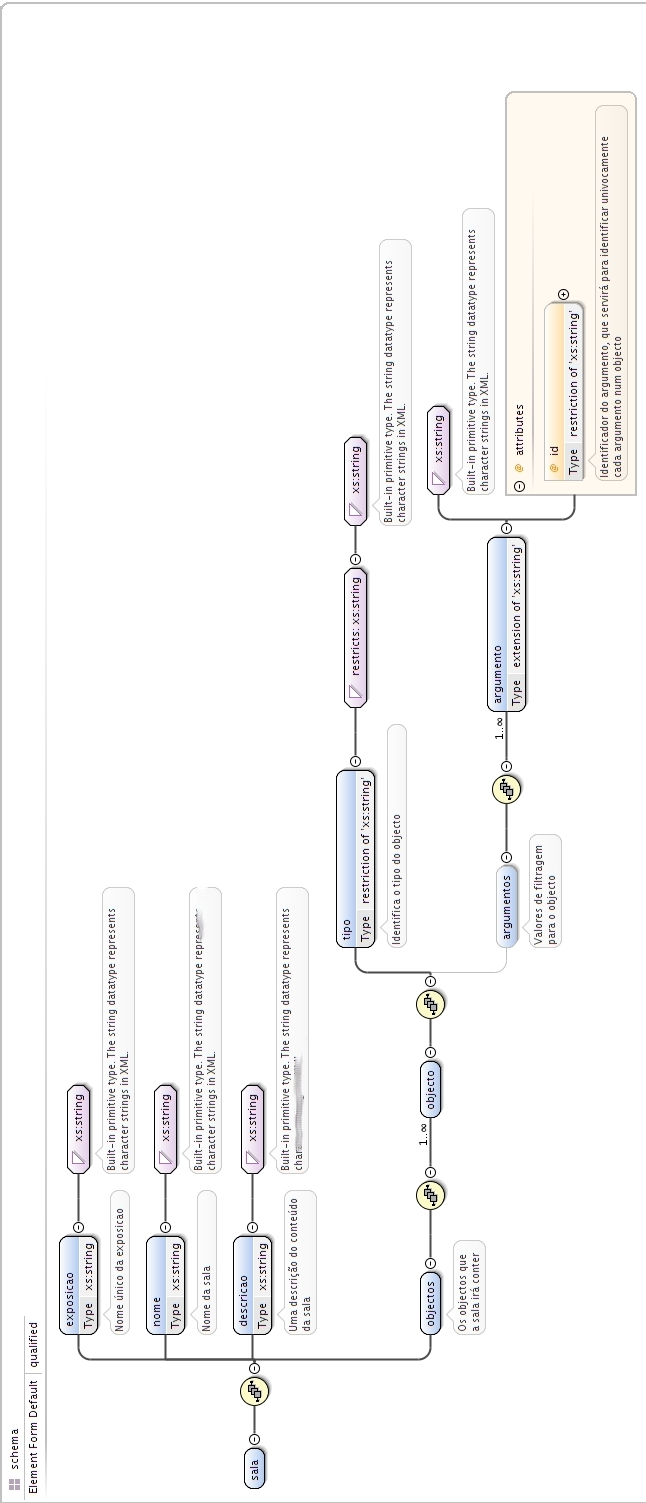
\includegraphics[width=4.0299in,height=9.4in]{relatoriopartebruno-img1.jpg}
\end{center}
\end{document}
